Below the plan for the search and seizure task, coupled with the pictures and
their descriptions.

\section{Plan}
\label{s:scene-planning}

\begin{enumerate}
  \item \textbf{Safety:} A bedroom is the subject of the examination. It is a
  double bedroom owned by a single person, meaning that control measures for
  entering or leaving the room are not followed.
  \item \textbf{Scene:} The scene setting as previously mentioned is for a
  double bedroom. It has two desks with desktop computers and general hardwares
  such as keyboards, mouses and monitors. A TV is also present on the right side
  of the room. A super-king bed is also found in the middle of the scene.
  \item \textbf{Assistance:} If large items need to be kept in costudy, then
  assistance would be required in order for the item to be taken in custody. For
  small devices, even though they can be easily handled, assistance might still
  be needed to isolation and prevention of any kind of damage.
  \item \textbf{Inteview:} Some questions could be asked to the suspect, such
  as passwords or additional informations.
\end{enumerate}

\newpage
\section{Pictures of Scene}
\label{s:scene-pictures}
In this section, all pictures related to the investigation are listed and
described.

\subsection{Full Scene}
\label{s:scene-full}
The picture below pictures the whole scene that is subject to the investigation.
\begin{figure}[h]
  \centering
  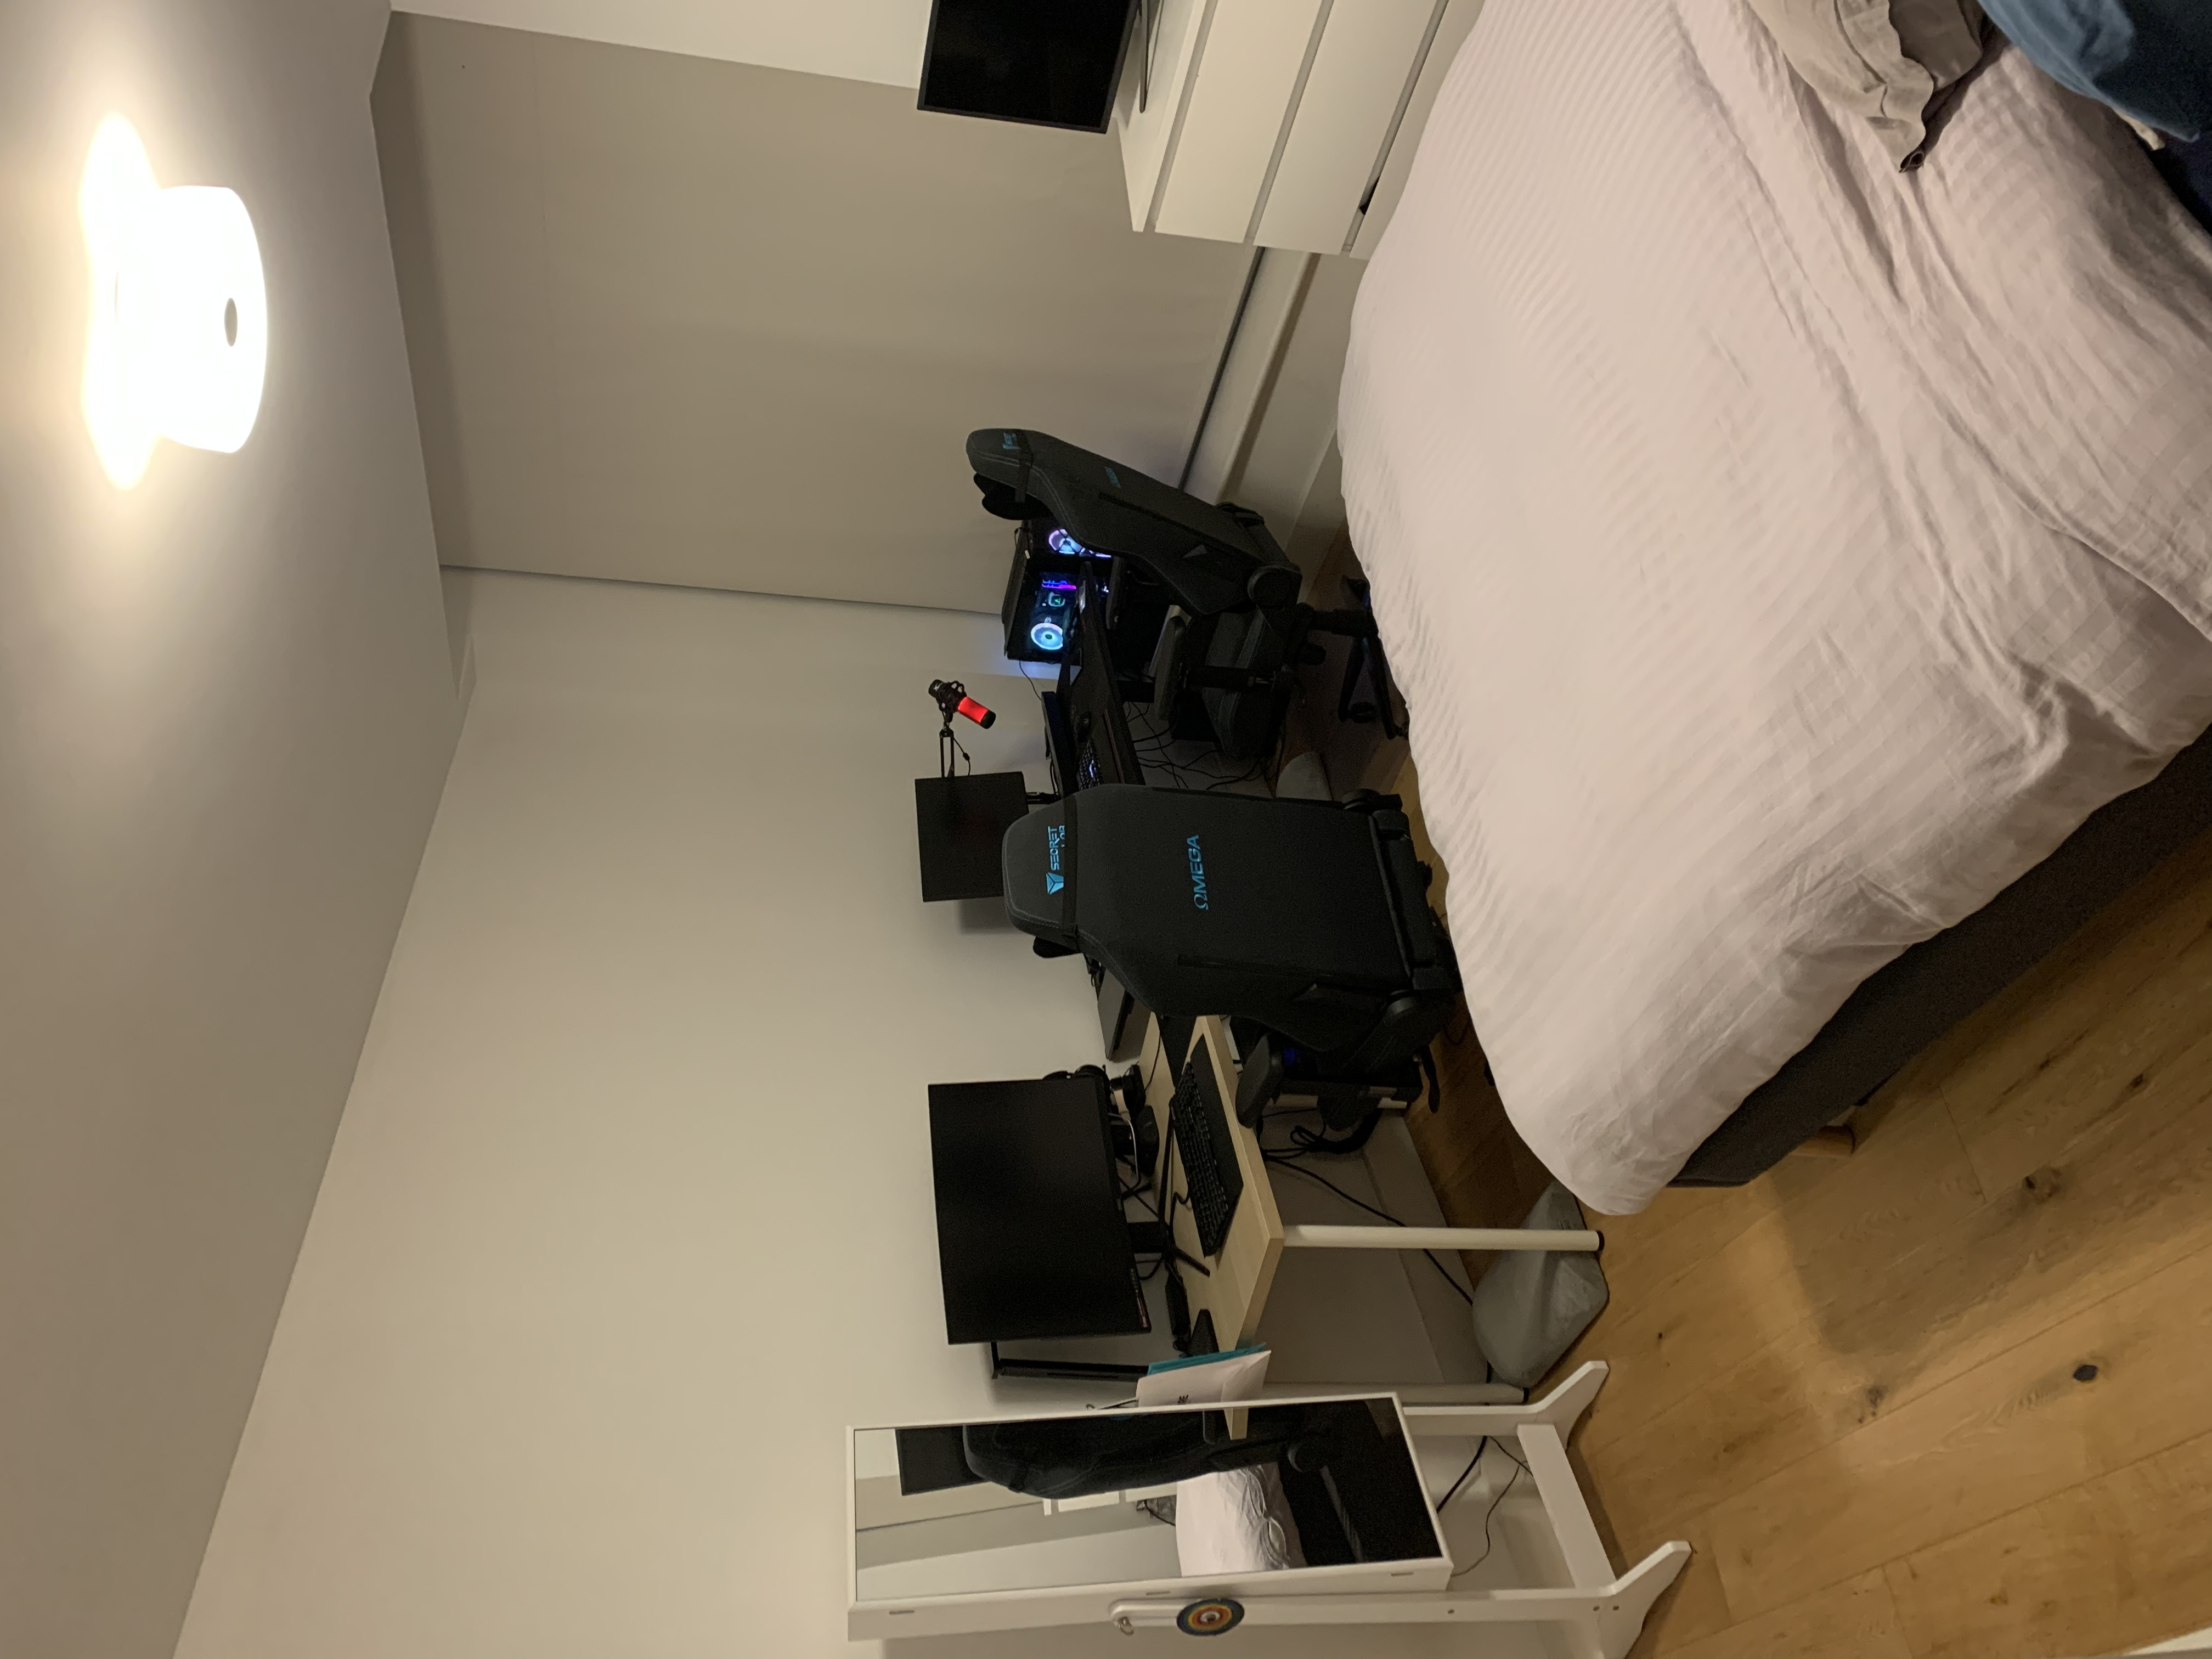
\includegraphics[width=0.8\textwidth, angle=-90,origin=c]{figures/pictures/IMG_5033.JPG}
  \caption{Full scene of the investigation}
  \label{fig:scene-full}
\end{figure}
\newpage

\subsection{Left Desk}
\label{s:left-desk}
The picture below shows the left desk of the scene. It has a monitor, speakers,
keyboard, mouse, mousepad and an Apple Watch. The Apple Watch has been taken
into custody for further investigation. See AB/5 (\ref{s:ab5}).
\begin{figure}[h]
  \centering
  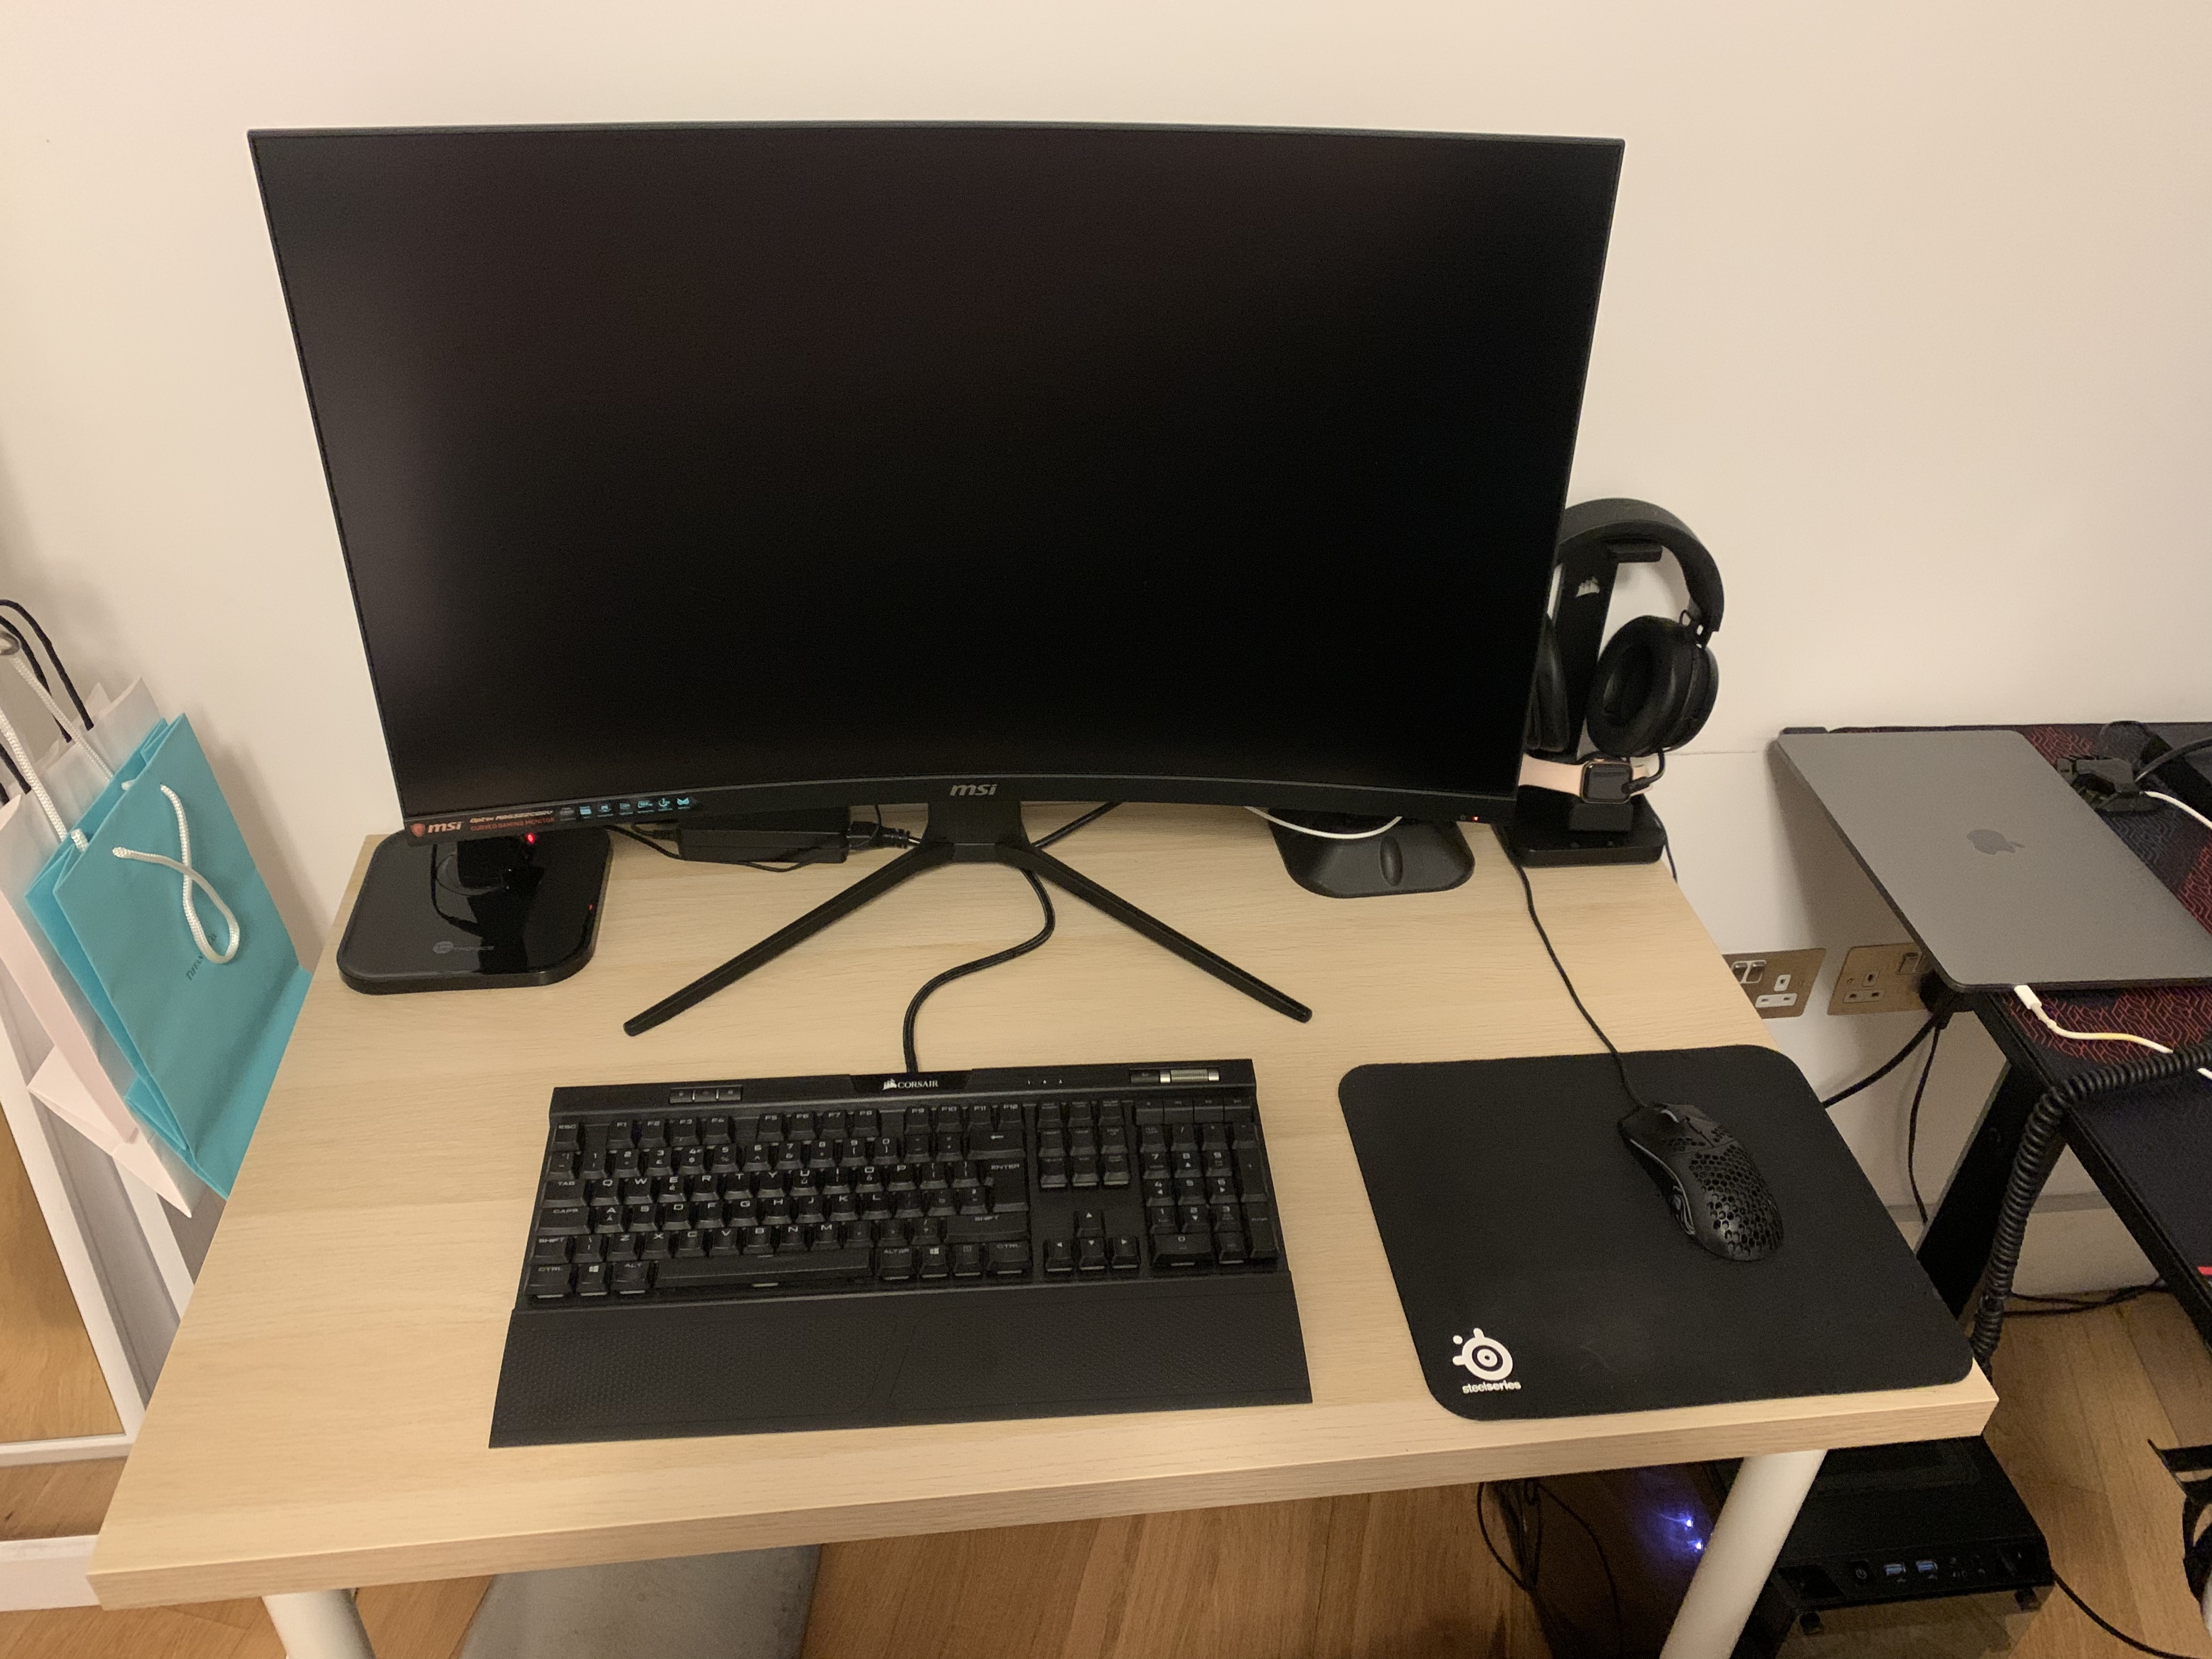
\includegraphics[width=0.8\textwidth]{figures/pictures/IMG_5036.JPG}
  \caption{Left Desk}
  \label{fig:left-desk}
\end{figure}
\newpage

\subsection{Right Desk}
\label{s:right-desk}
The picture below shows the right desk of the scene. It has a monitor, speakers,
keyboard, mouse, mousepad, microphone, laptop, HDD, soundbar, subwoofer,
controller, an amp sound card and a smartphone. The items taken in costudy are
the Laptop (\ref{s:ab1}), HDD (\ref{s:ab2}) and the smartphone (\ref{s:ab3}).
\begin{figure}[h]
  \centering
  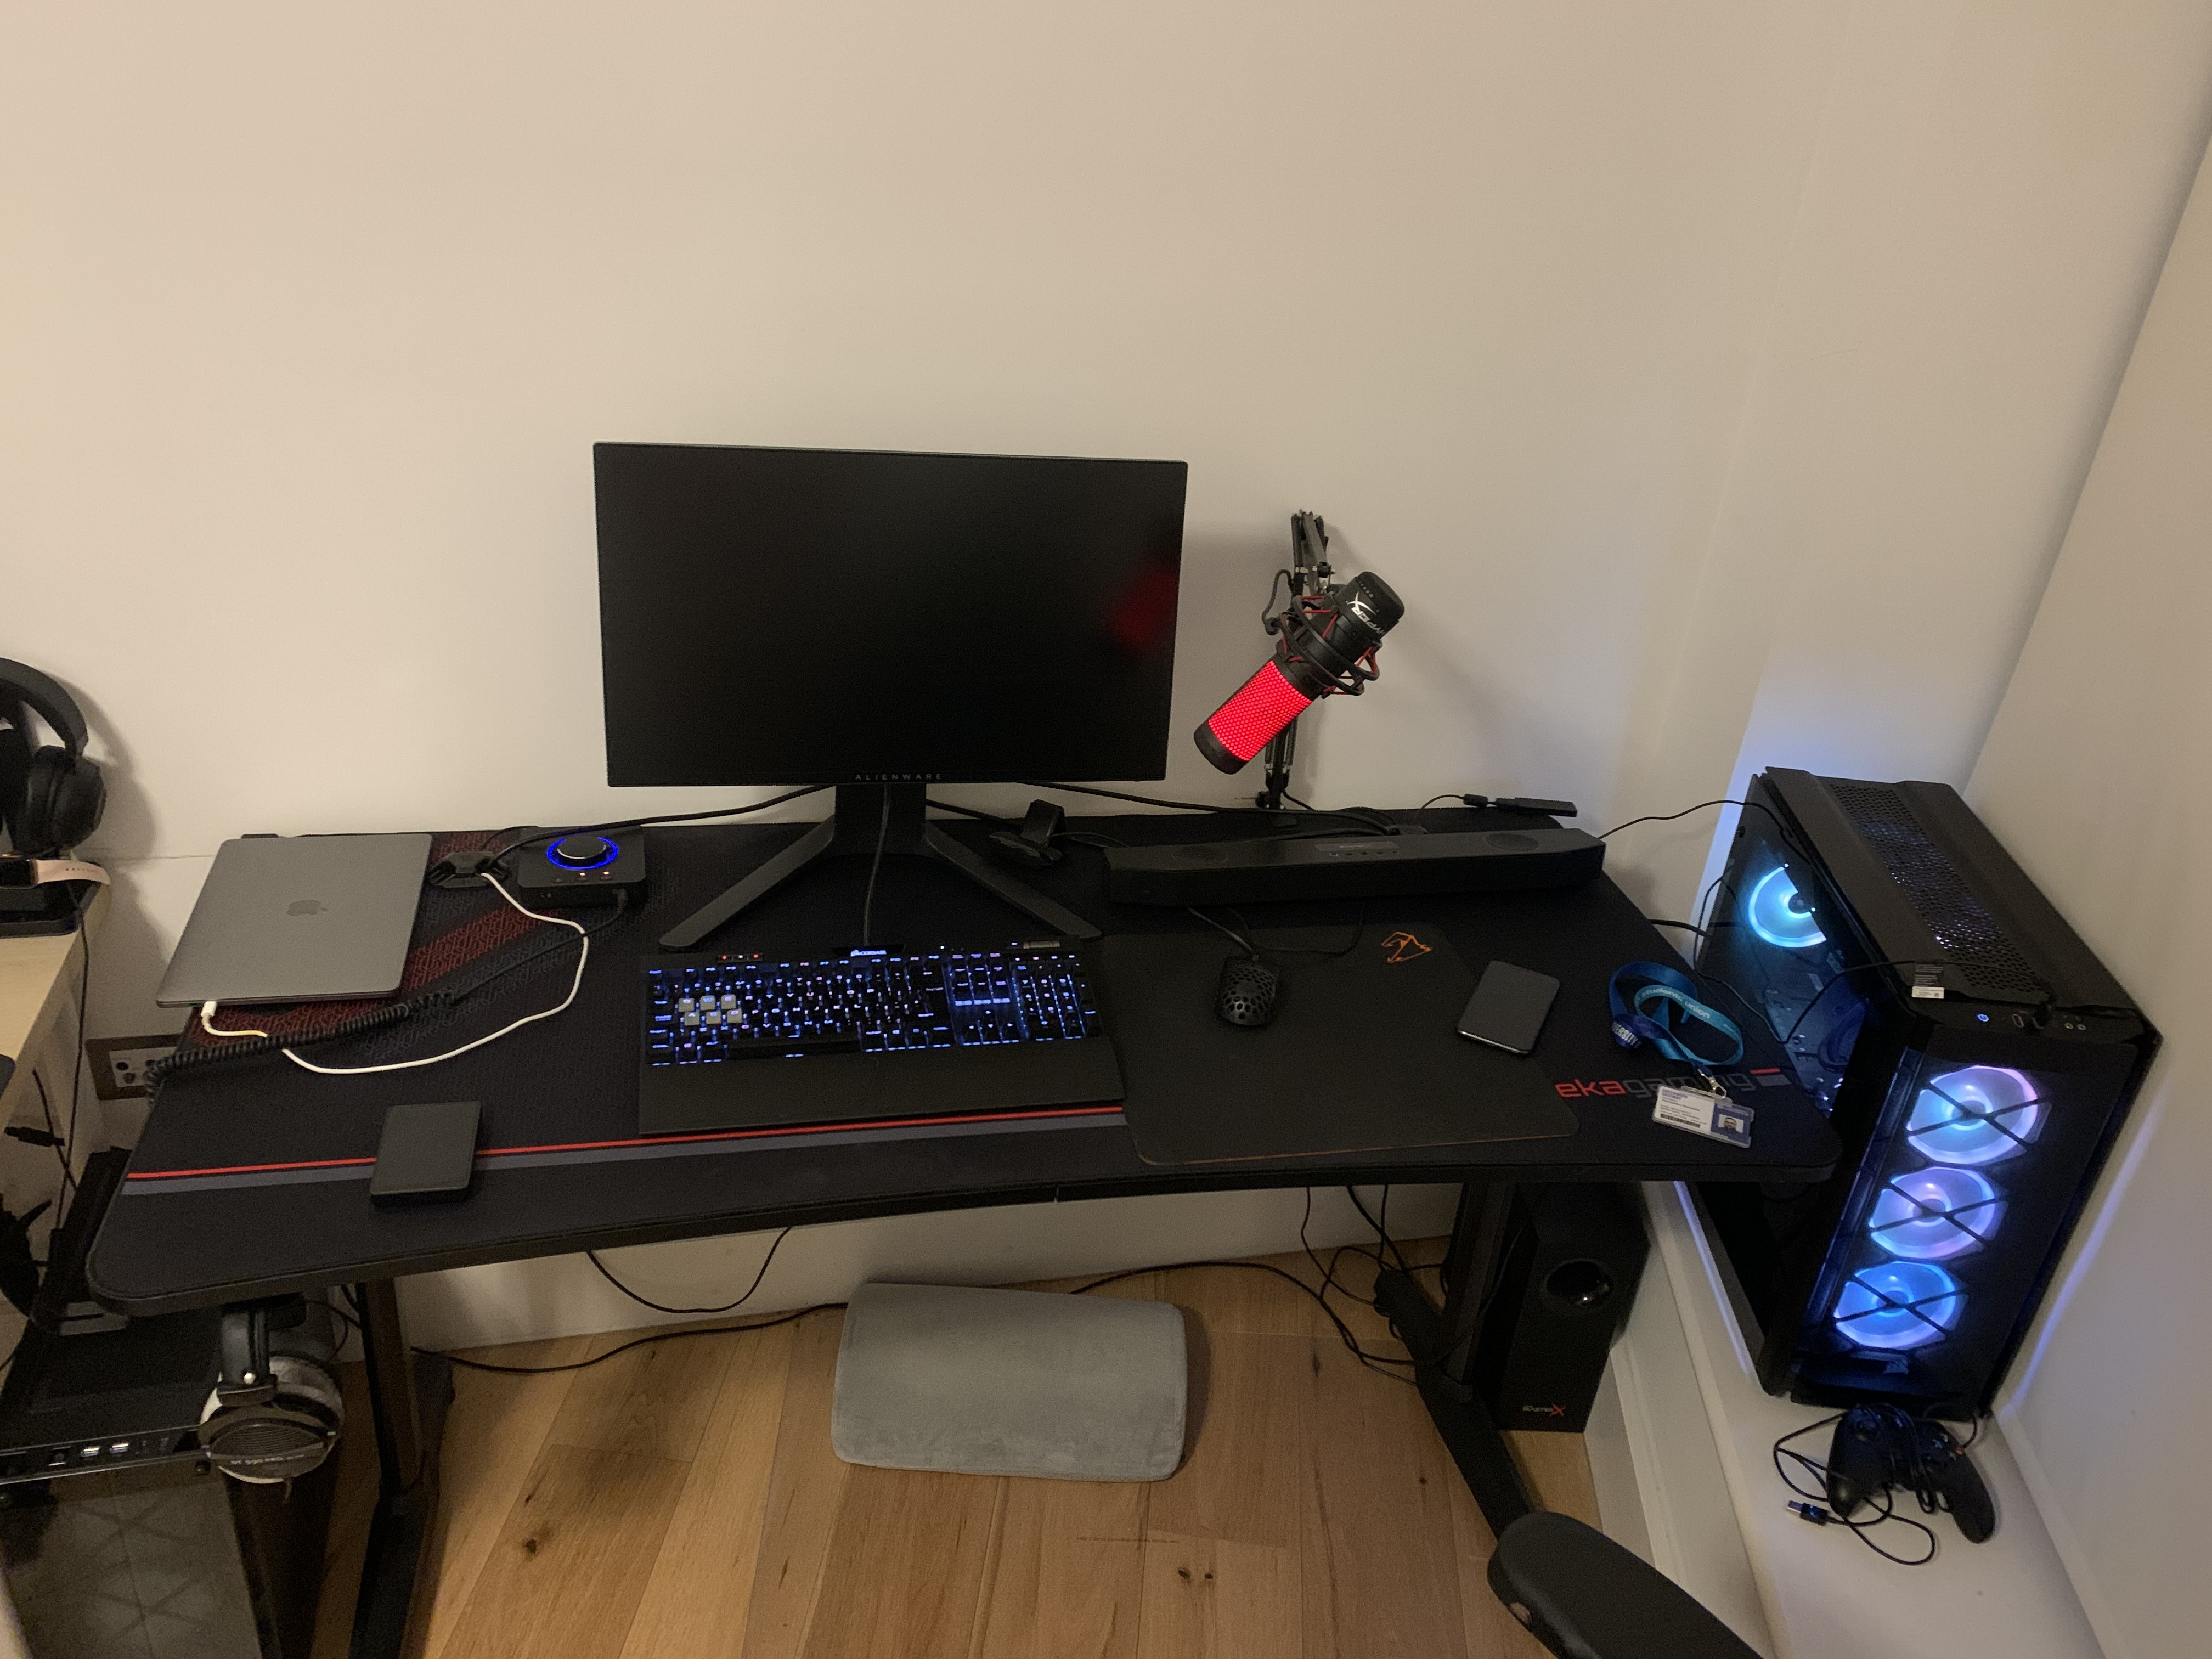
\includegraphics[width=0.8\textwidth]{figures/pictures/IMG_5038.JPG}
  \caption{Right Desk}
  \label{fig:right-desk}
\end{figure}
\newpage

\subsection{Chest of Drawer}
\label{s:drawer}
The picture below shows a chest of drawers used as a stand for a TV\@. On top of
it there is also a portable usb that has been taken in custody (AB/4).
\begin{figure}[h]
  \centering
  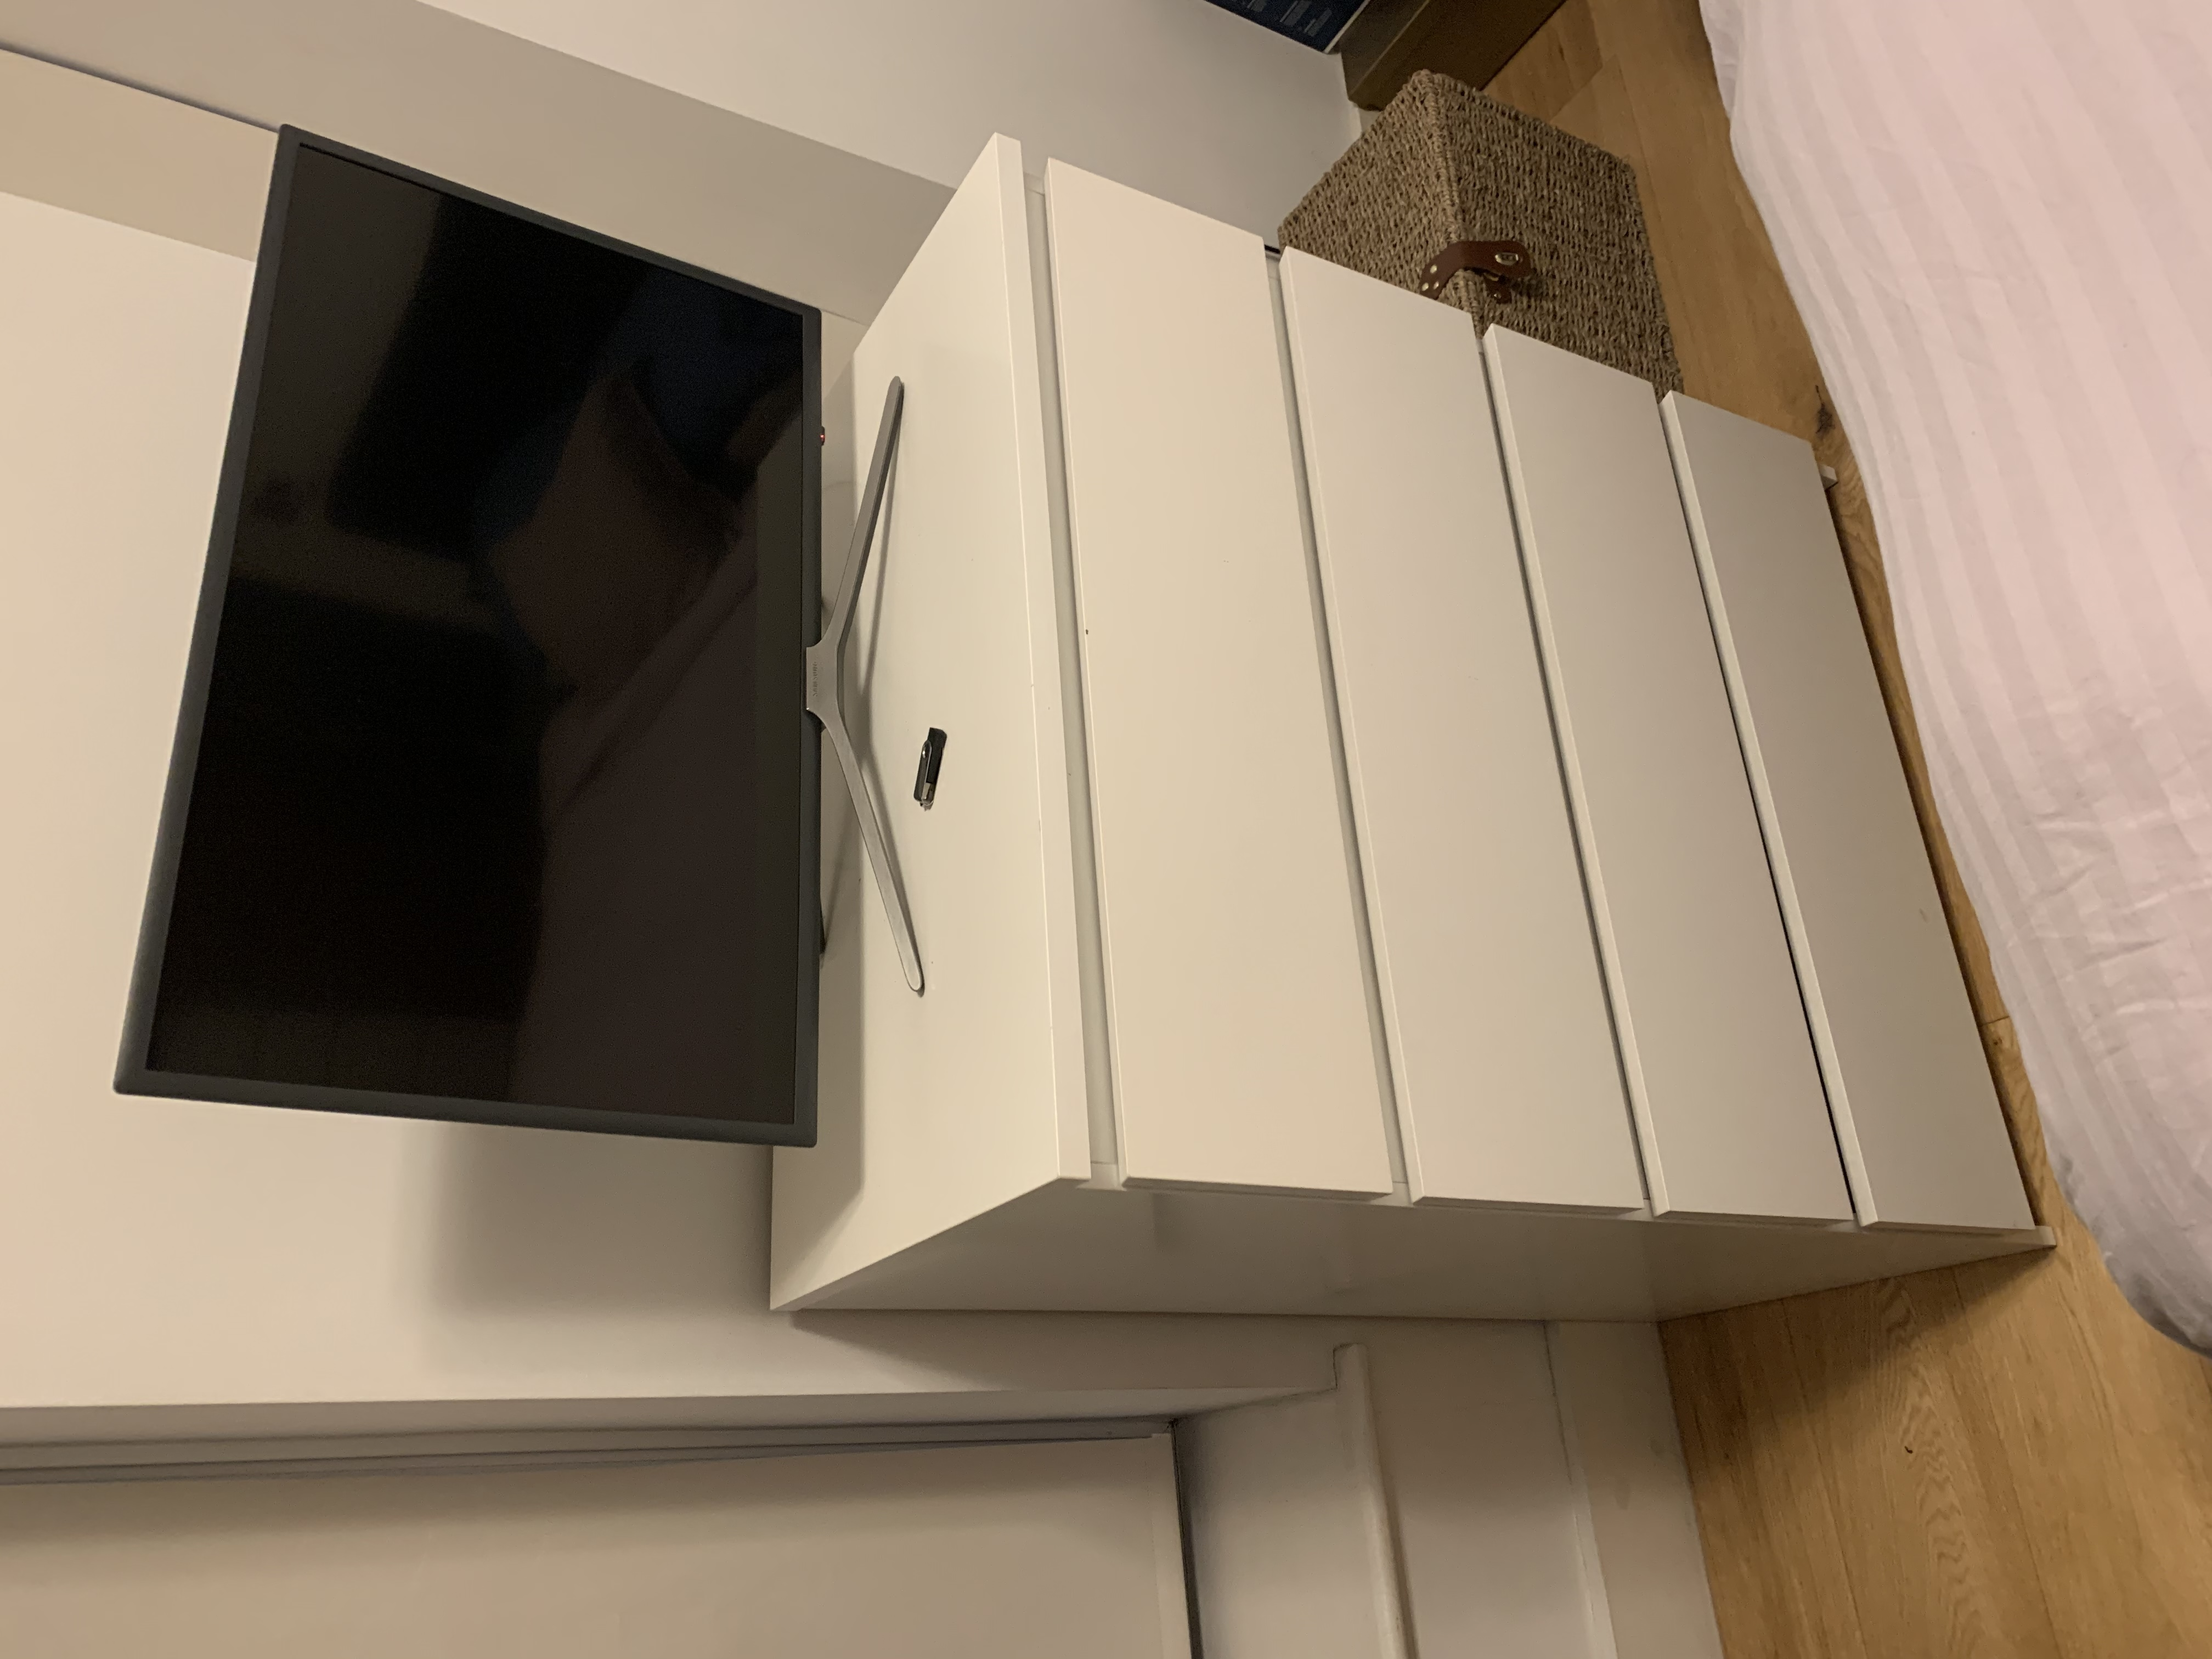
\includegraphics[width=0.8\textwidth, angle=-90,origin=c]{figures/pictures/IMG_5039.JPG}
  \caption{Chest of Drawer with TV}
  \label{fig:drawer}
\end{figure}
\newpage
\section{Pictures of Evidences}
\label{s:evidence-pictures}
In this section, all pictures of the evidences that have been taken in custody.

\subsection{Exhibit AB/1 (MacBook Pro)}
\label{s:ab1}

\begin{figure}[h]
  \centering
  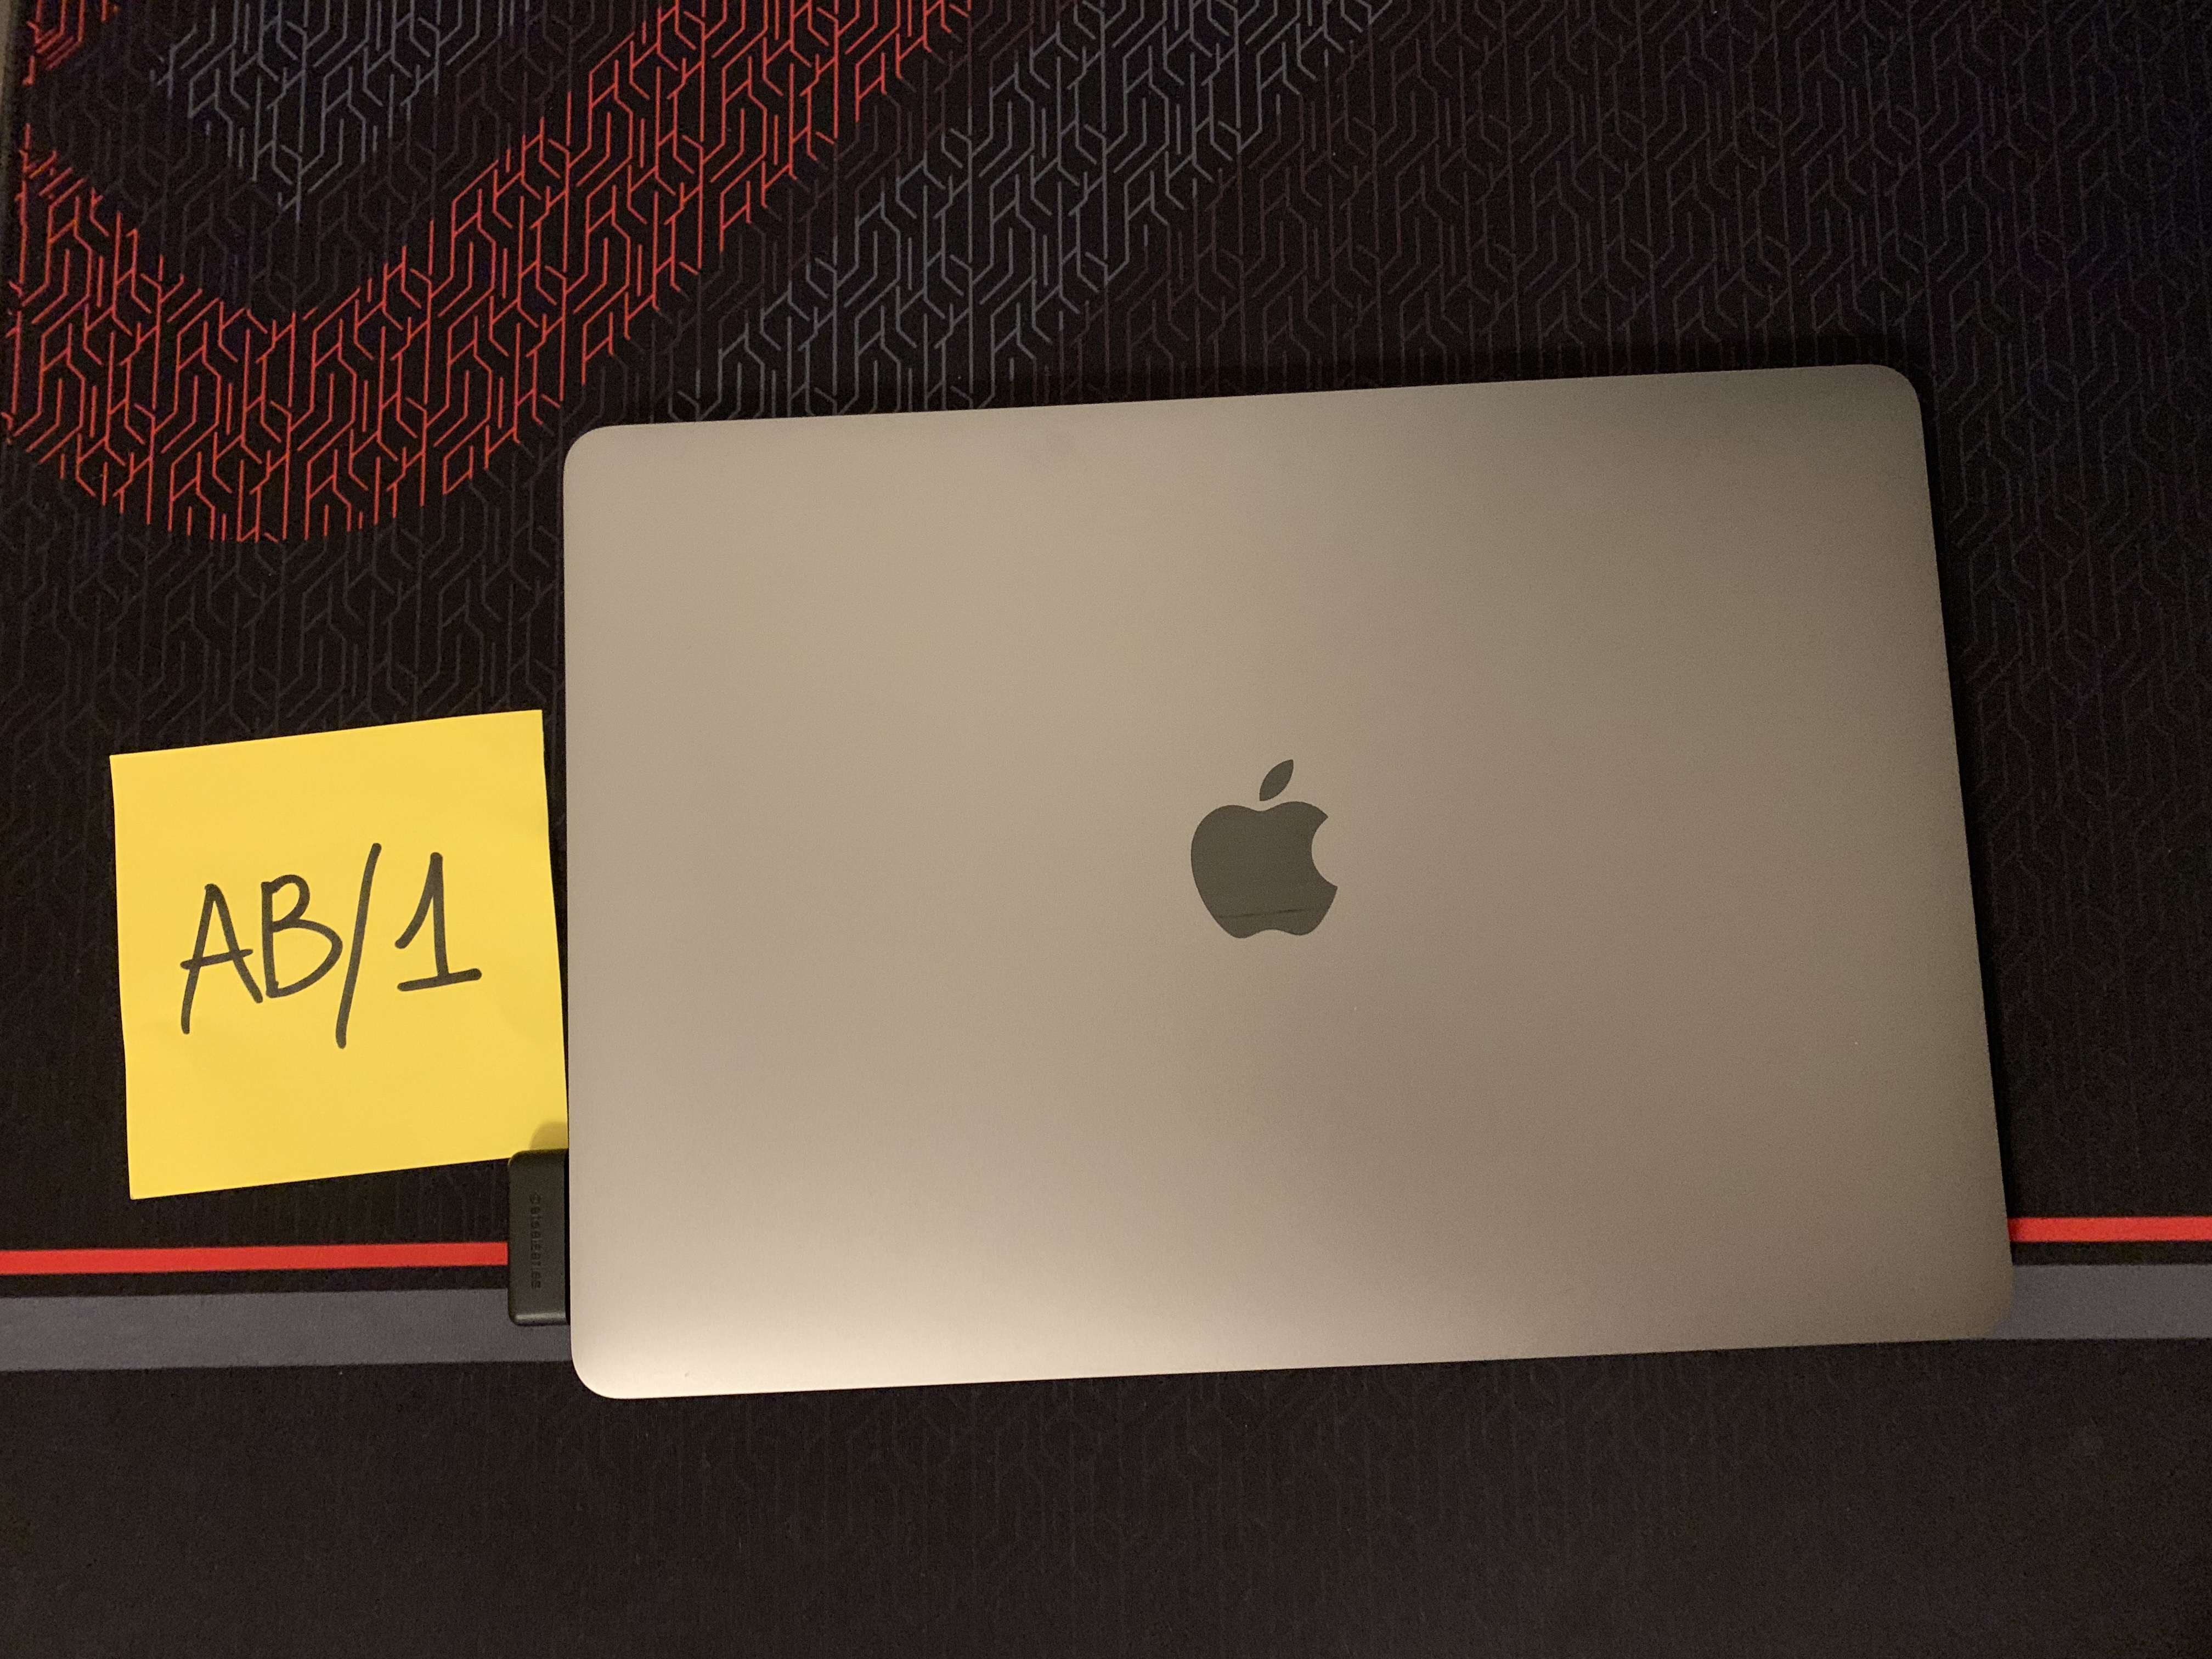
\includegraphics[width=0.7\textwidth]{figures/pictures/IMG_5042.JPG}
  \caption{Macbook Pro: Front}
  \label{fig:macbook-front}
\end{figure}

\begin{figure}[h]
  \centering
  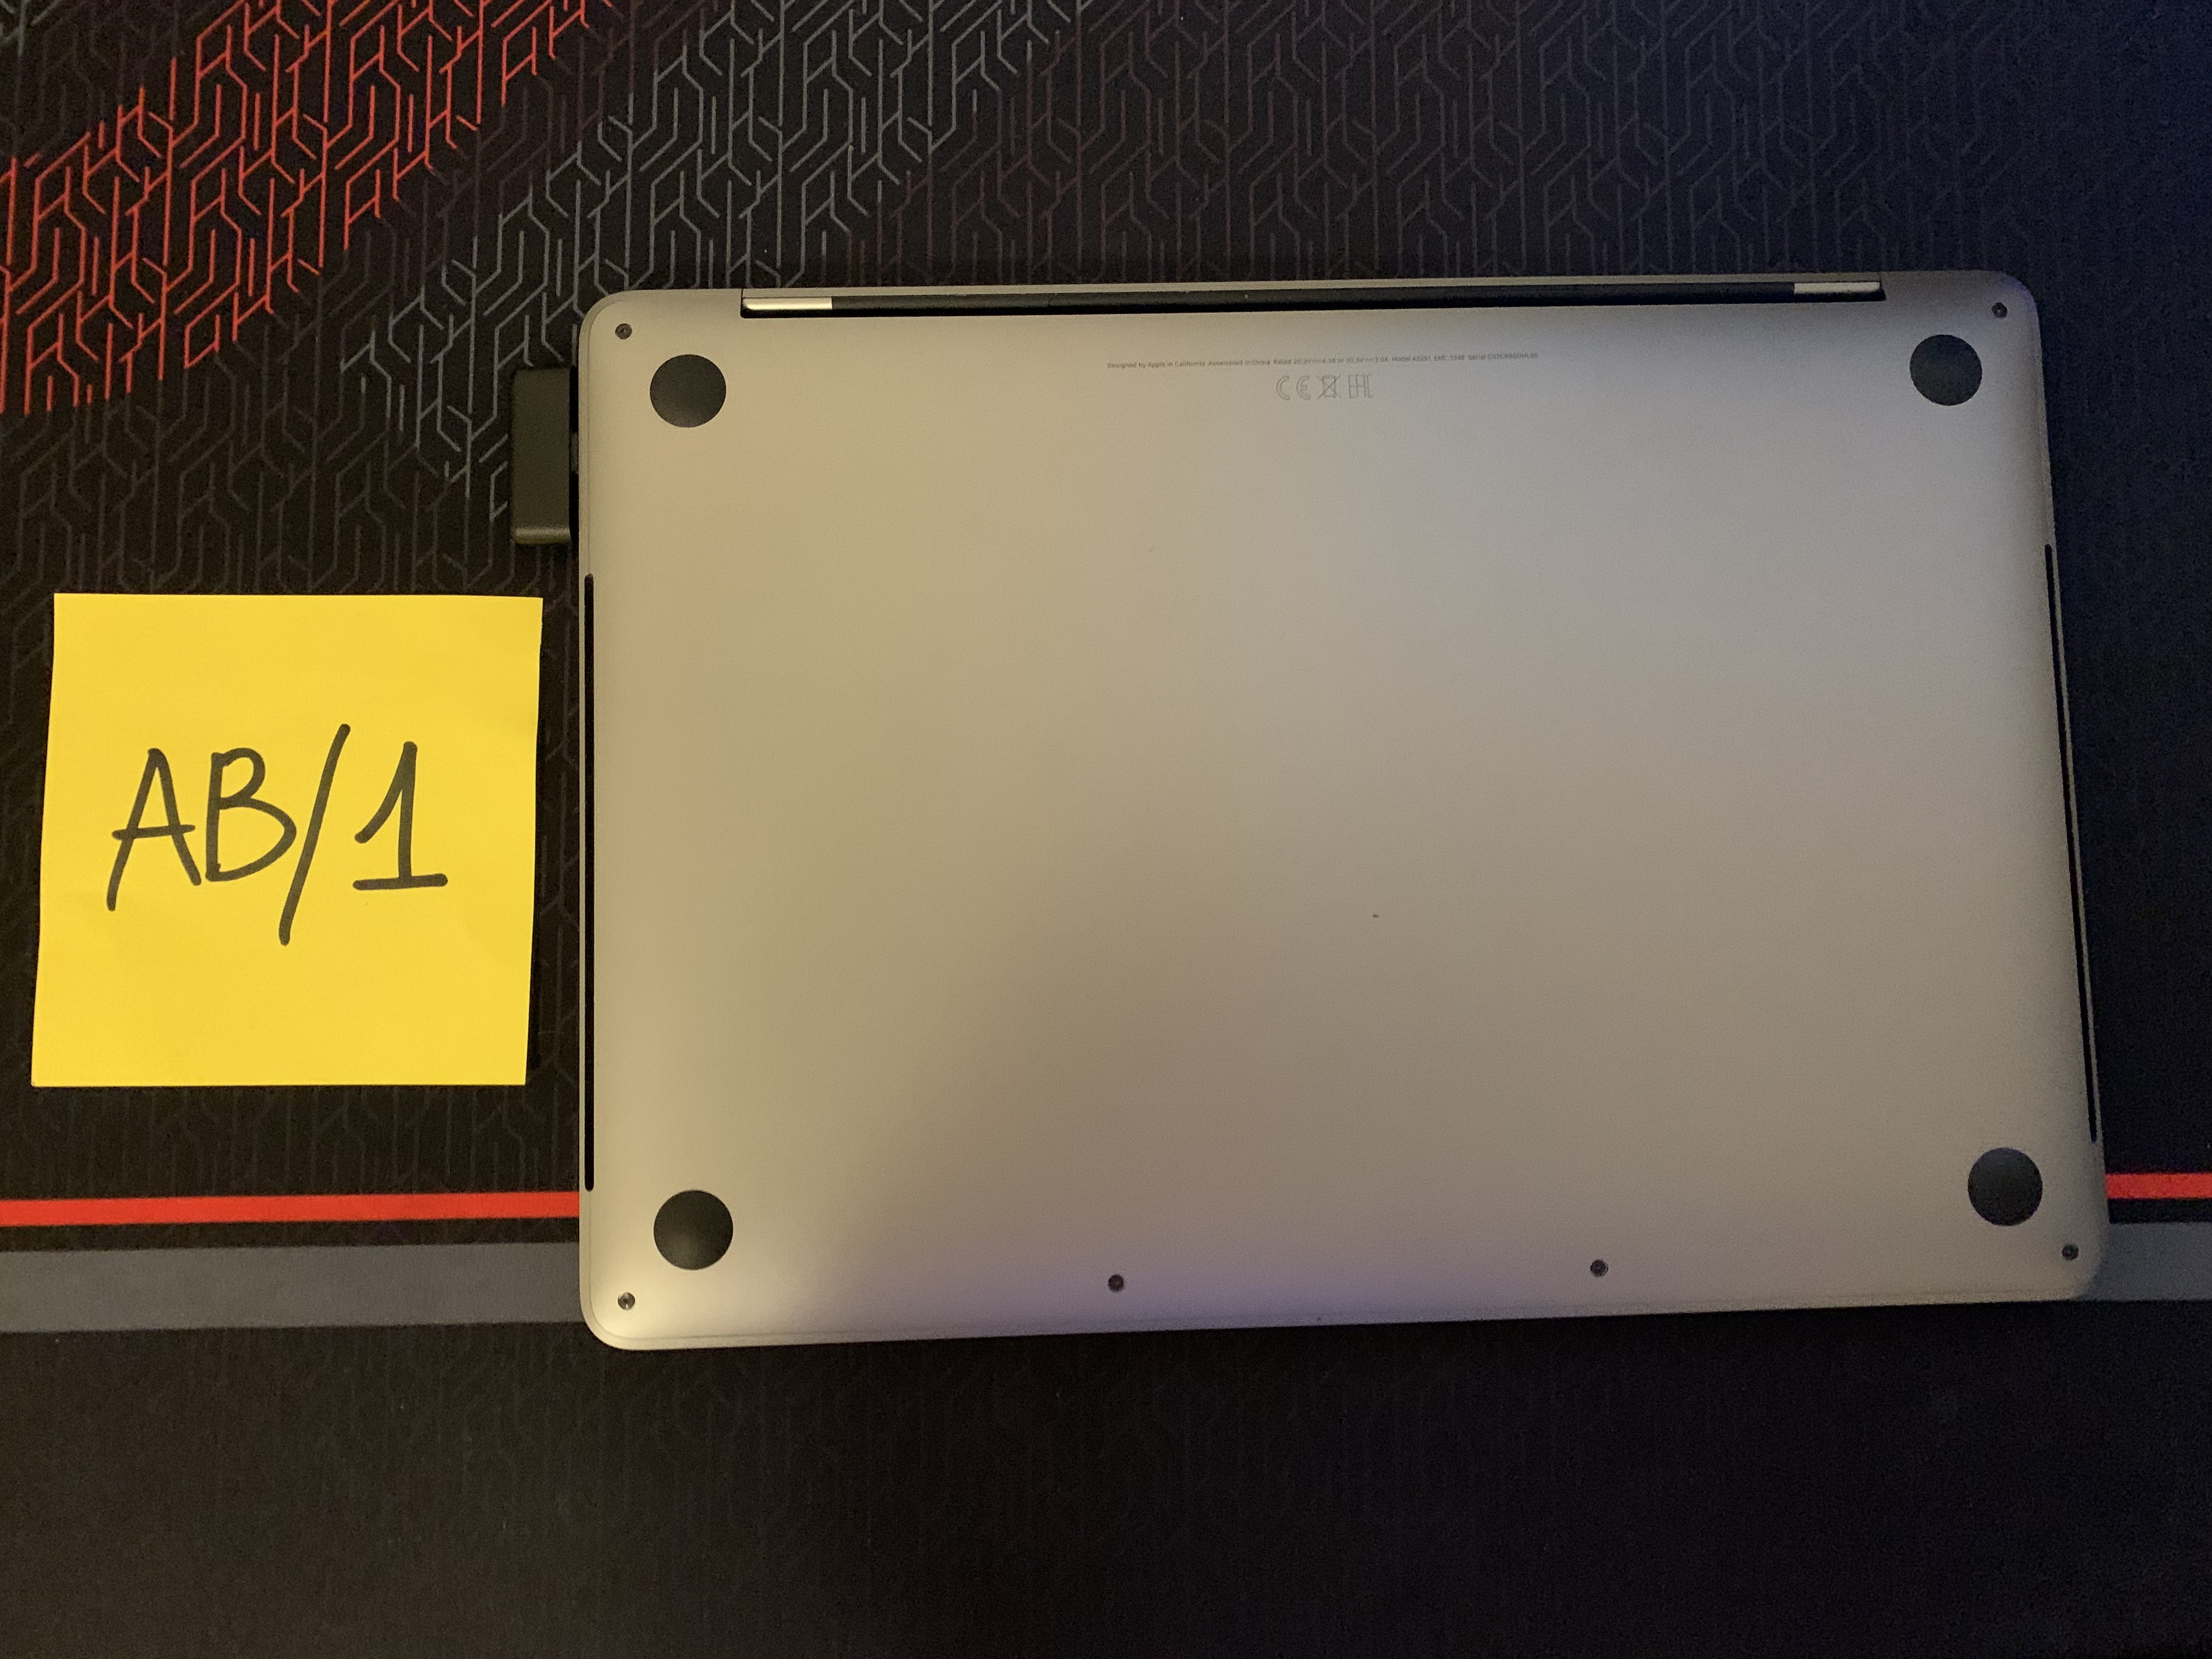
\includegraphics[width=0.7\textwidth]{figures/pictures/IMG_5043.JPG}
  \caption{Macbook Pro: Back}
  \label{fig:macbook-back}
\end{figure}
\newpage

\subsection{Exhibit AB/2 (HDD)}
\label{s:ab2}

\begin{figure}[h]
  \centering
  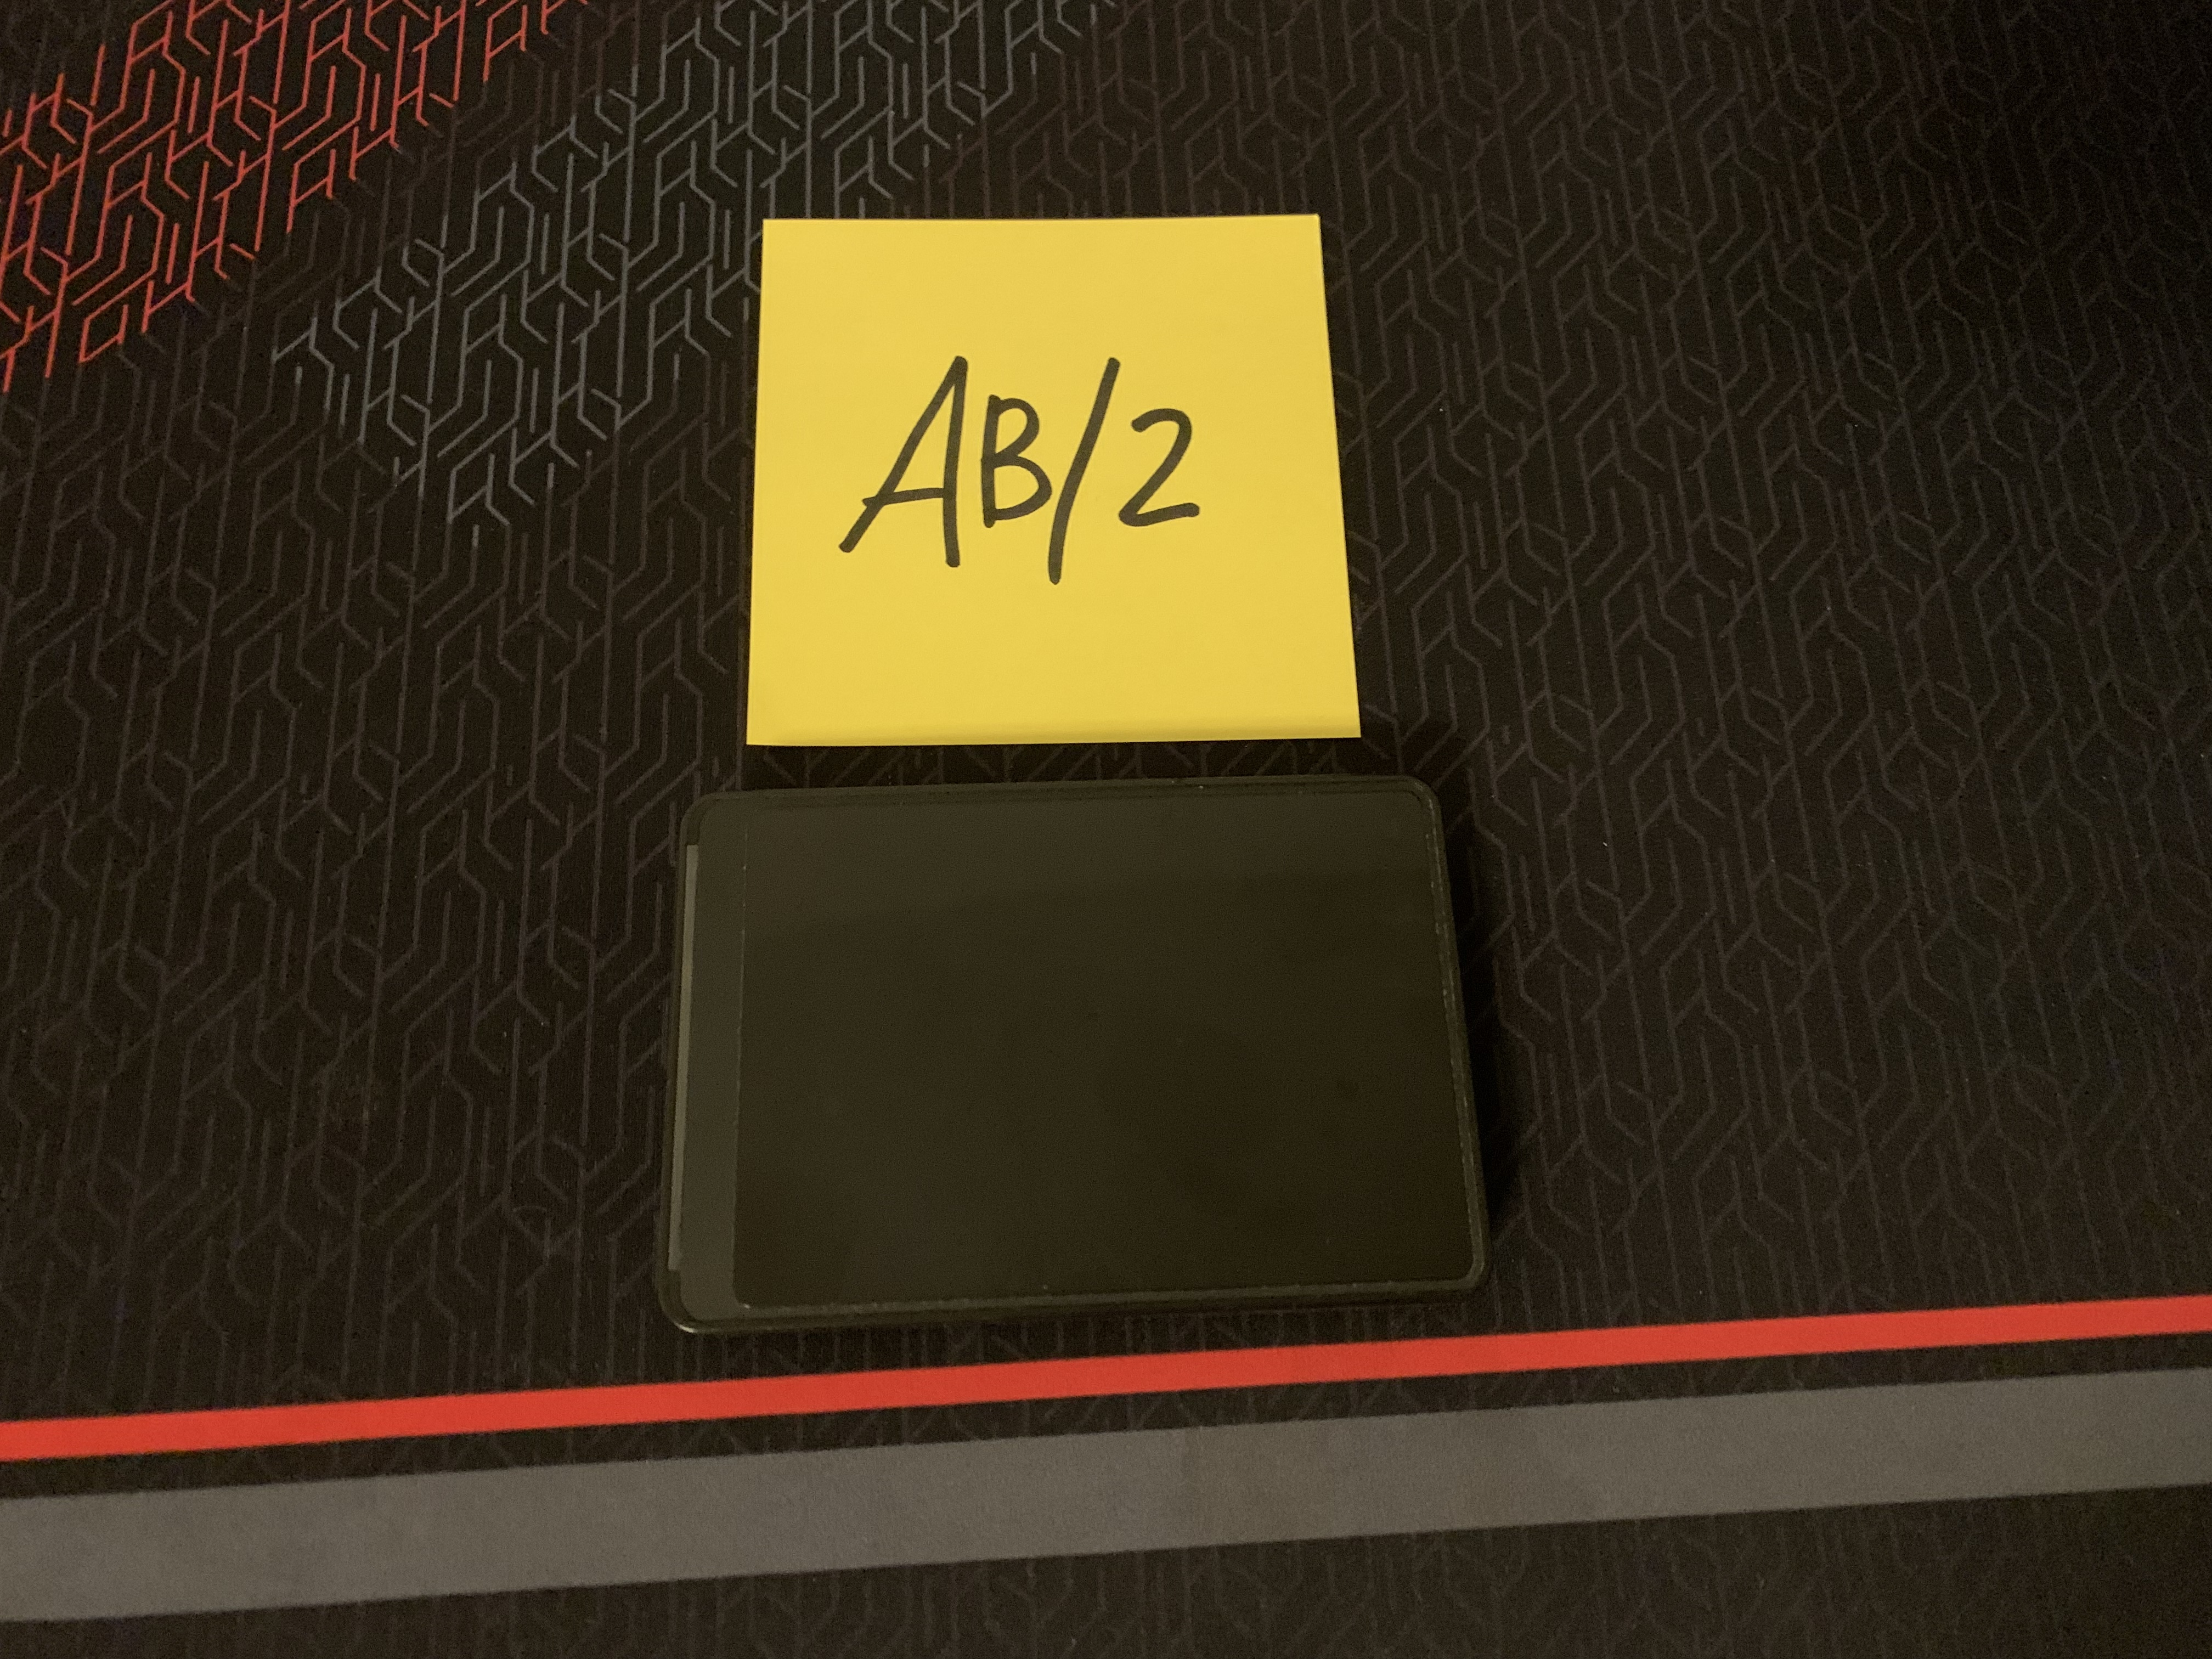
\includegraphics[width=0.7\textwidth]{figures/pictures/IMG_5044.JPG}
  \caption{HDD: Front}
  \label{fig:hdd-front}
\end{figure}

\begin{figure}[h]
  \centering
  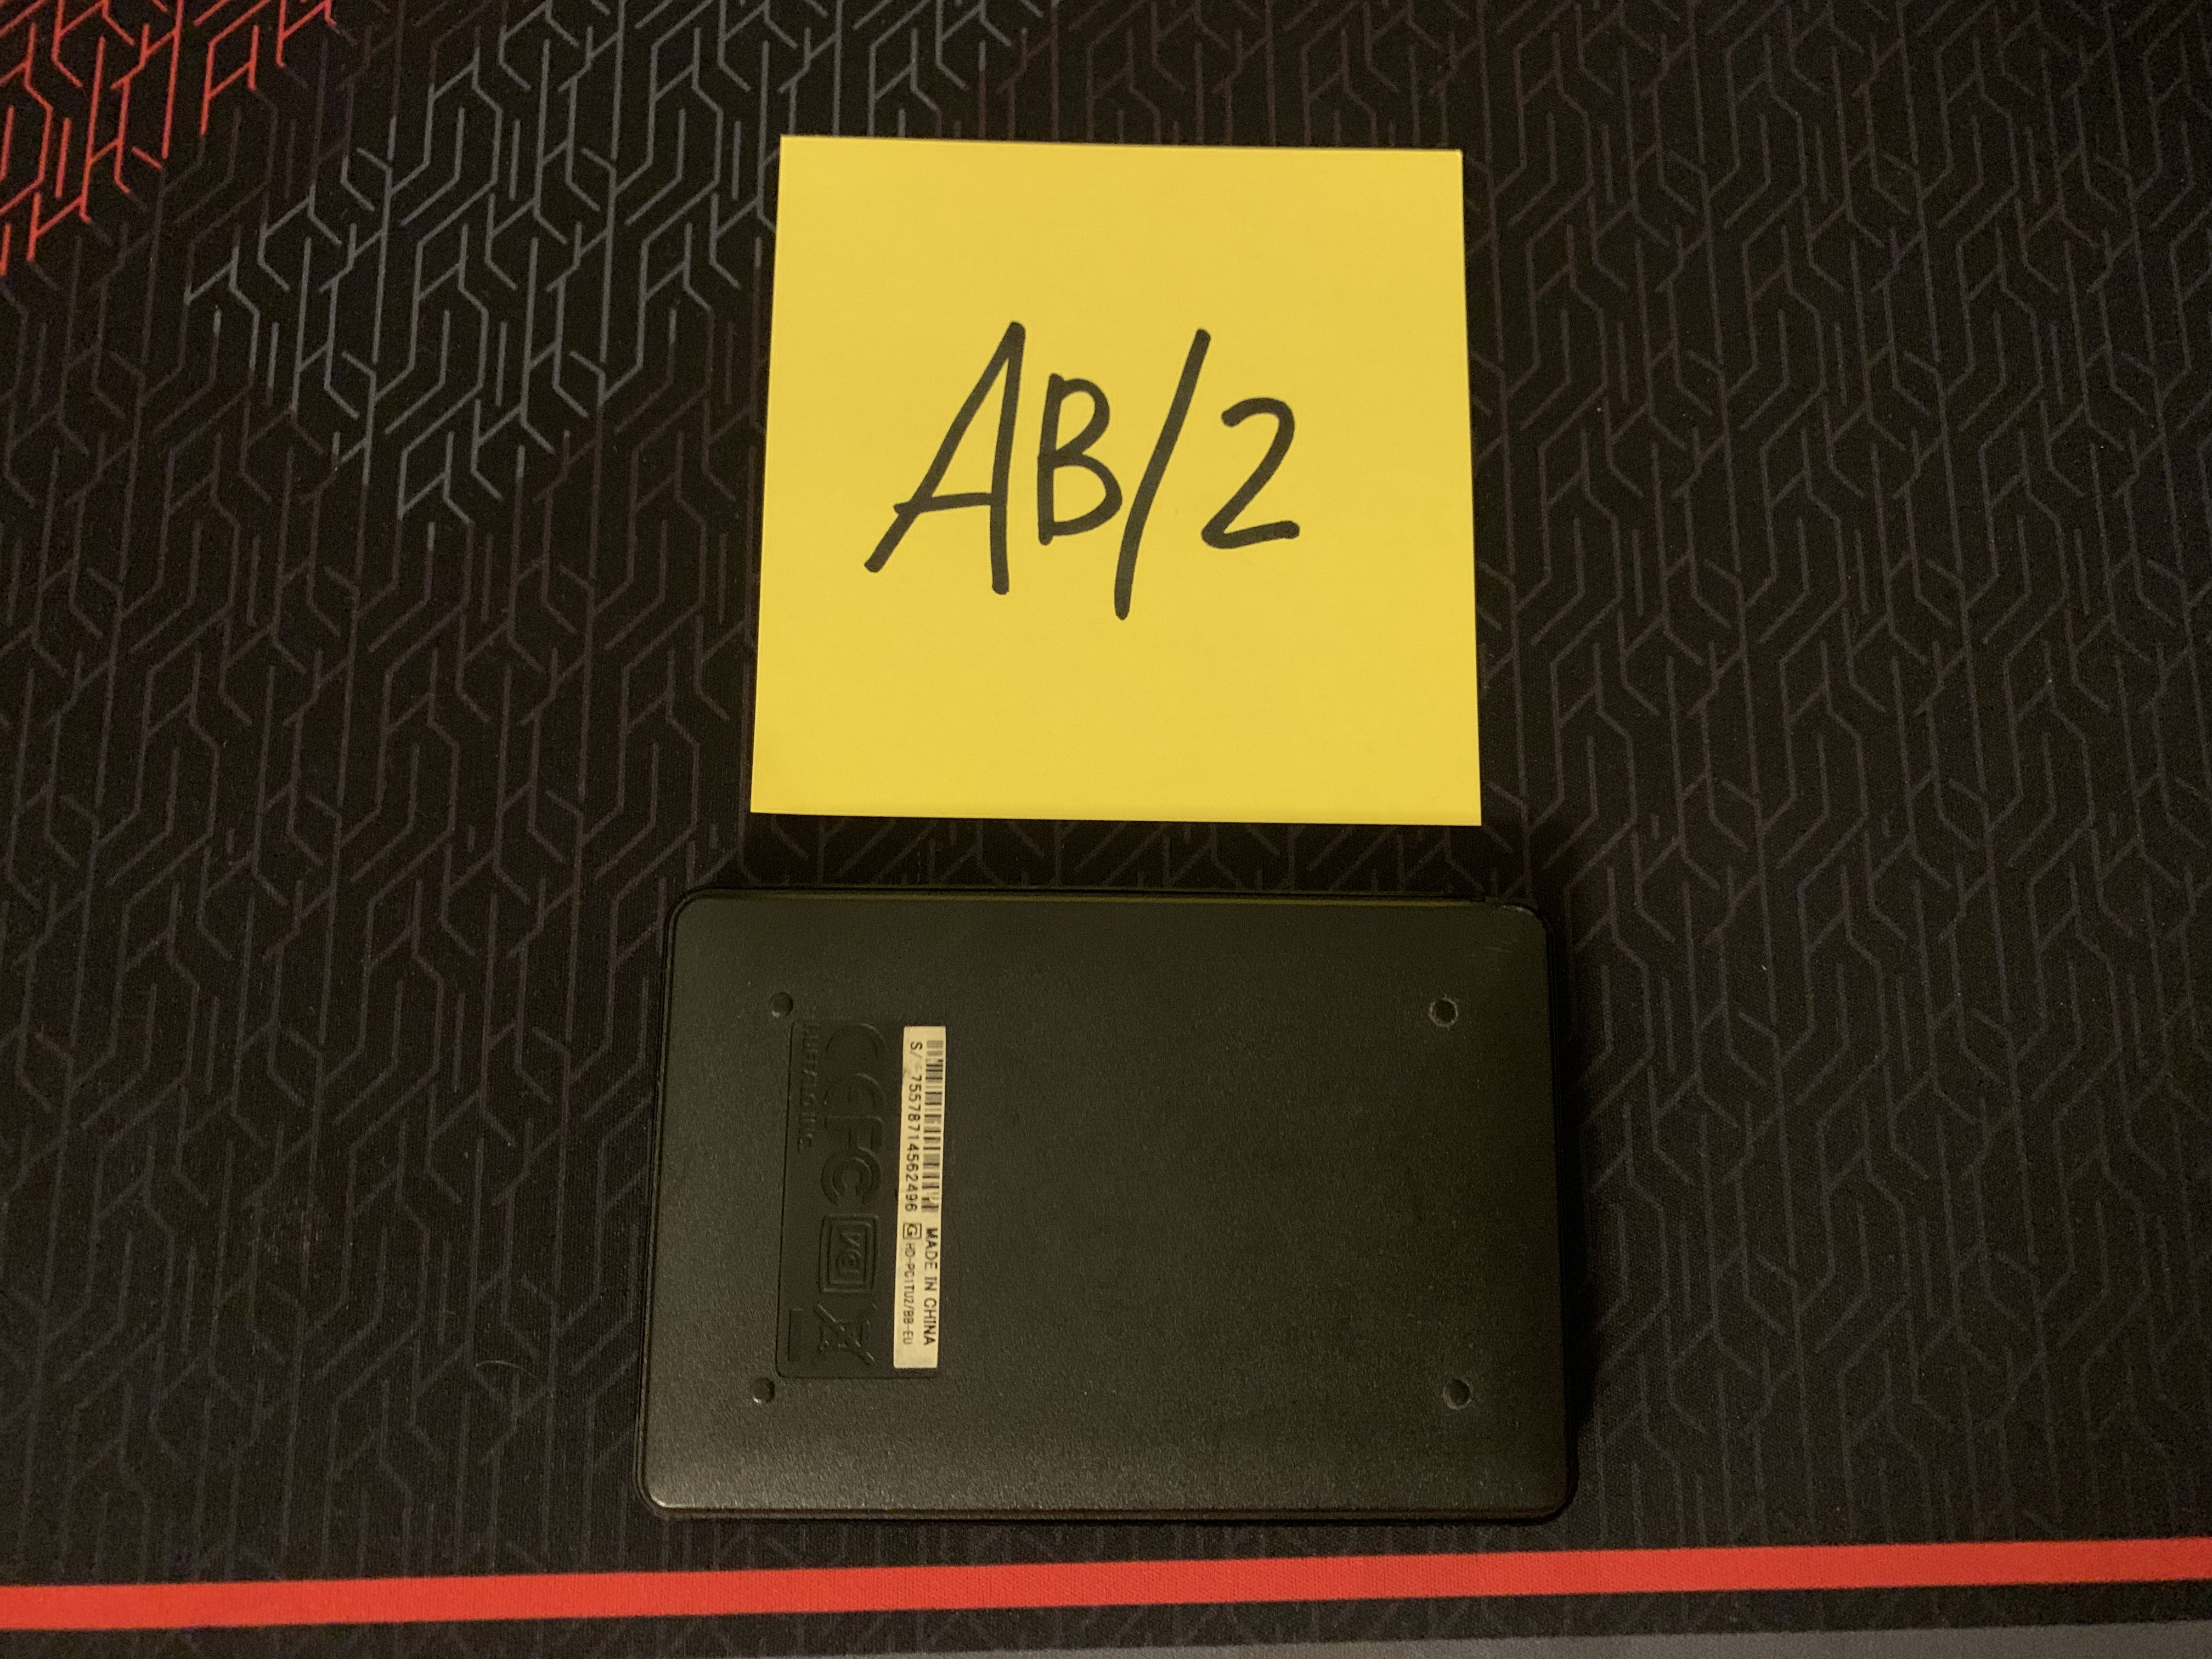
\includegraphics[width=0.7\textwidth]{figures/pictures/IMG_5045.JPG}
  \caption{HDD: Back}
  \label{fig:hdd-back}
\end{figure}
\newpage

\subsection{Exhibit AB/3 (Smartphone)}
\label{s:ab3}

\begin{figure}[h]
  \centering
  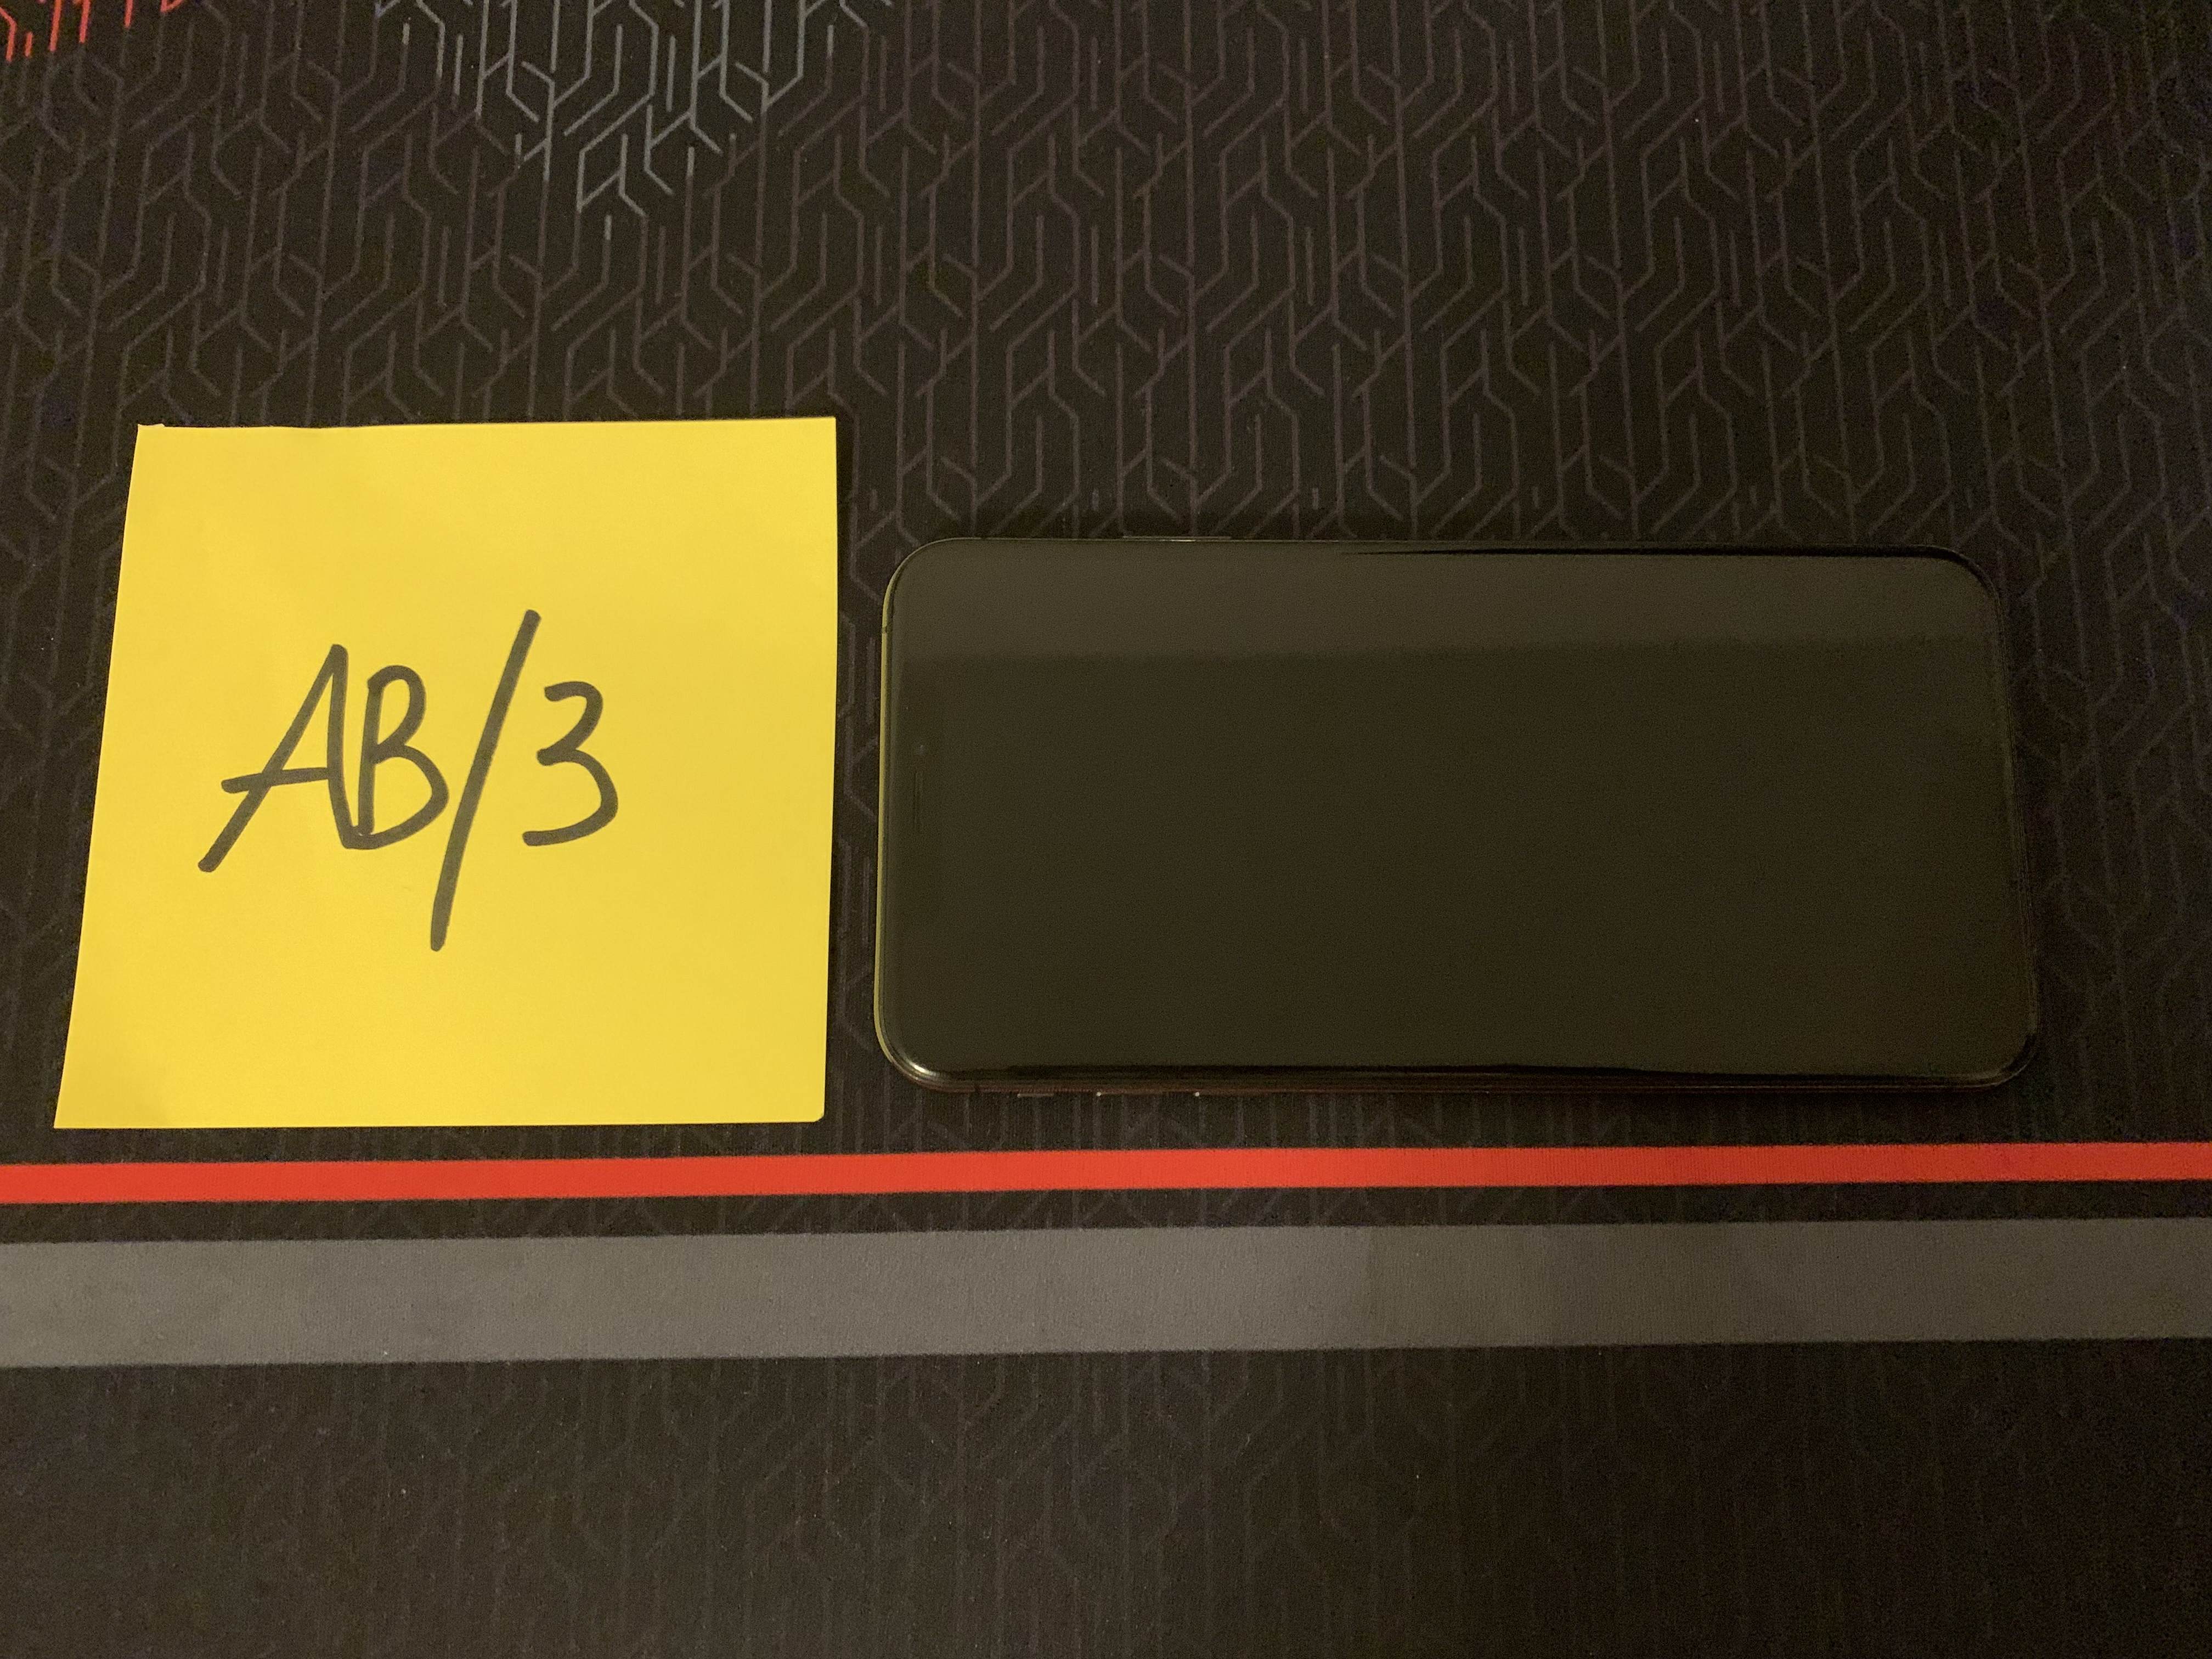
\includegraphics[width=0.7\textwidth]{figures/pictures/IMG_5046.JPG}
  \caption{Smartphone: Front}
  \label{fig:smartphone-front}
\end{figure}

\begin{figure}[h]
  \centering
  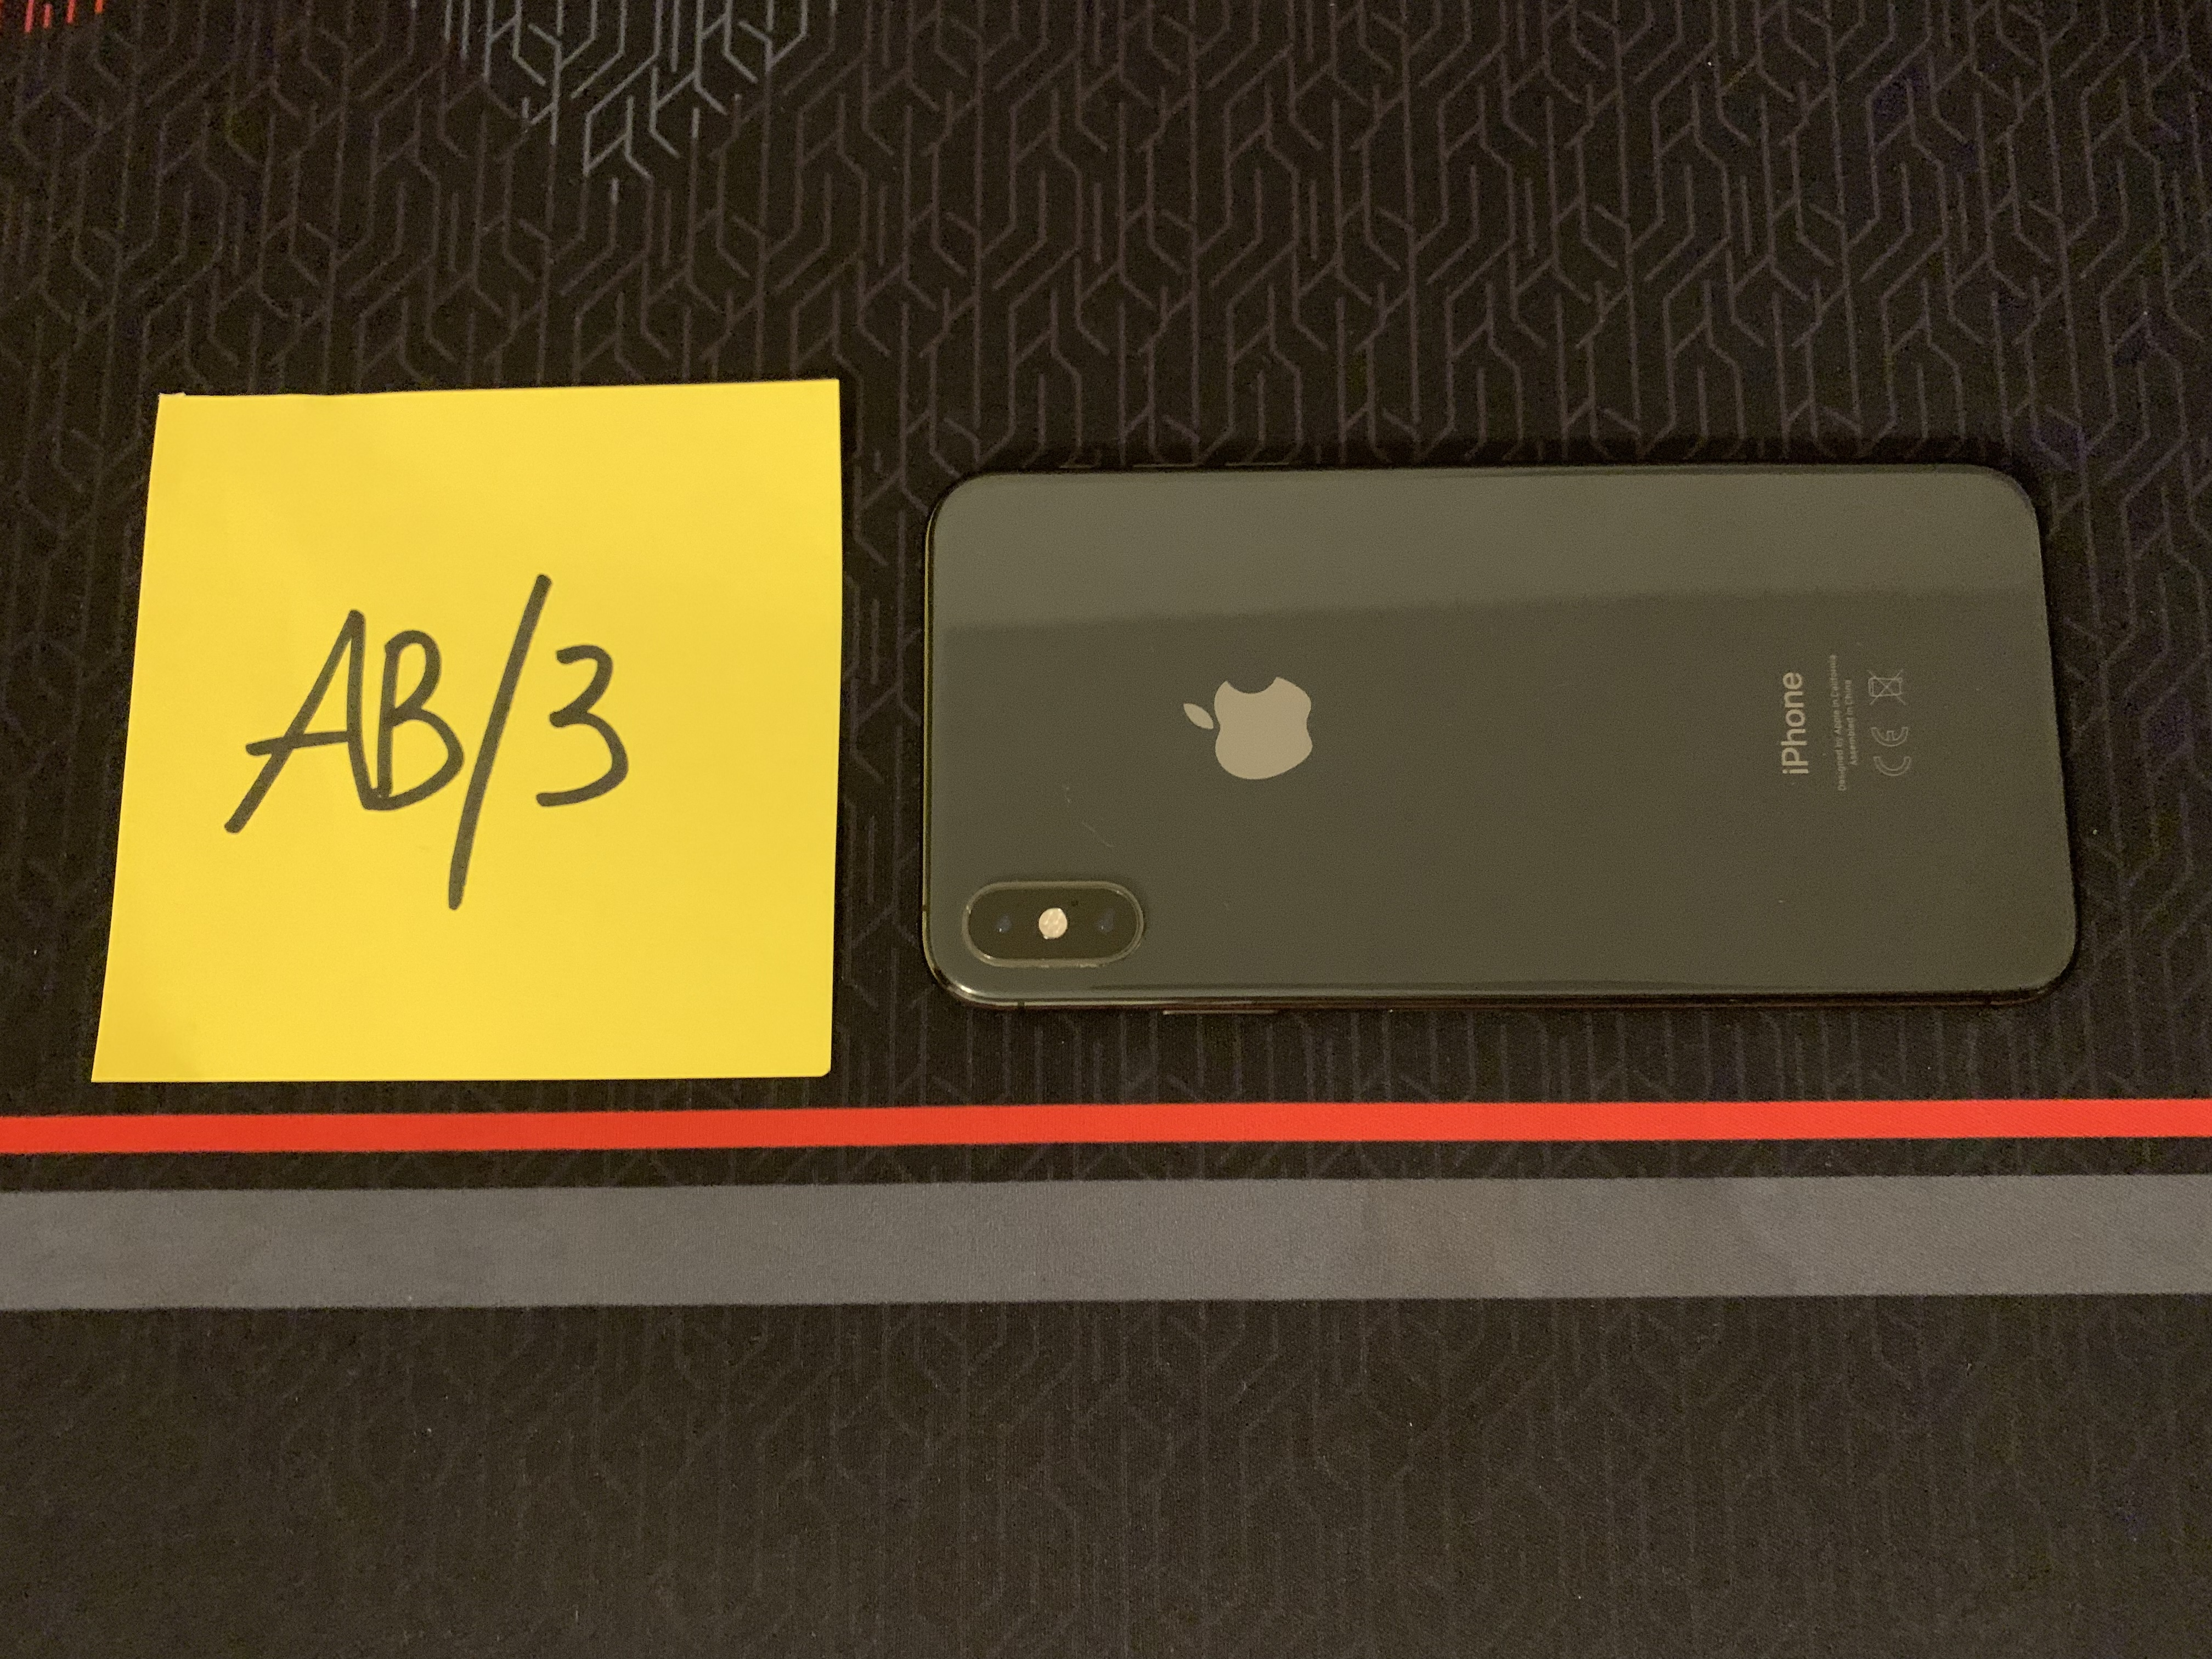
\includegraphics[width=0.7\textwidth]{figures/pictures/IMG_5047.JPG}
  \caption{Smartphone: Back}
  \label{fig:smartphone-back}
\end{figure}
\newpage

\subsection{Exhibit AB/4 (Portable USB)}
\label{s:ab4}

\begin{figure}[h]
  \centering
  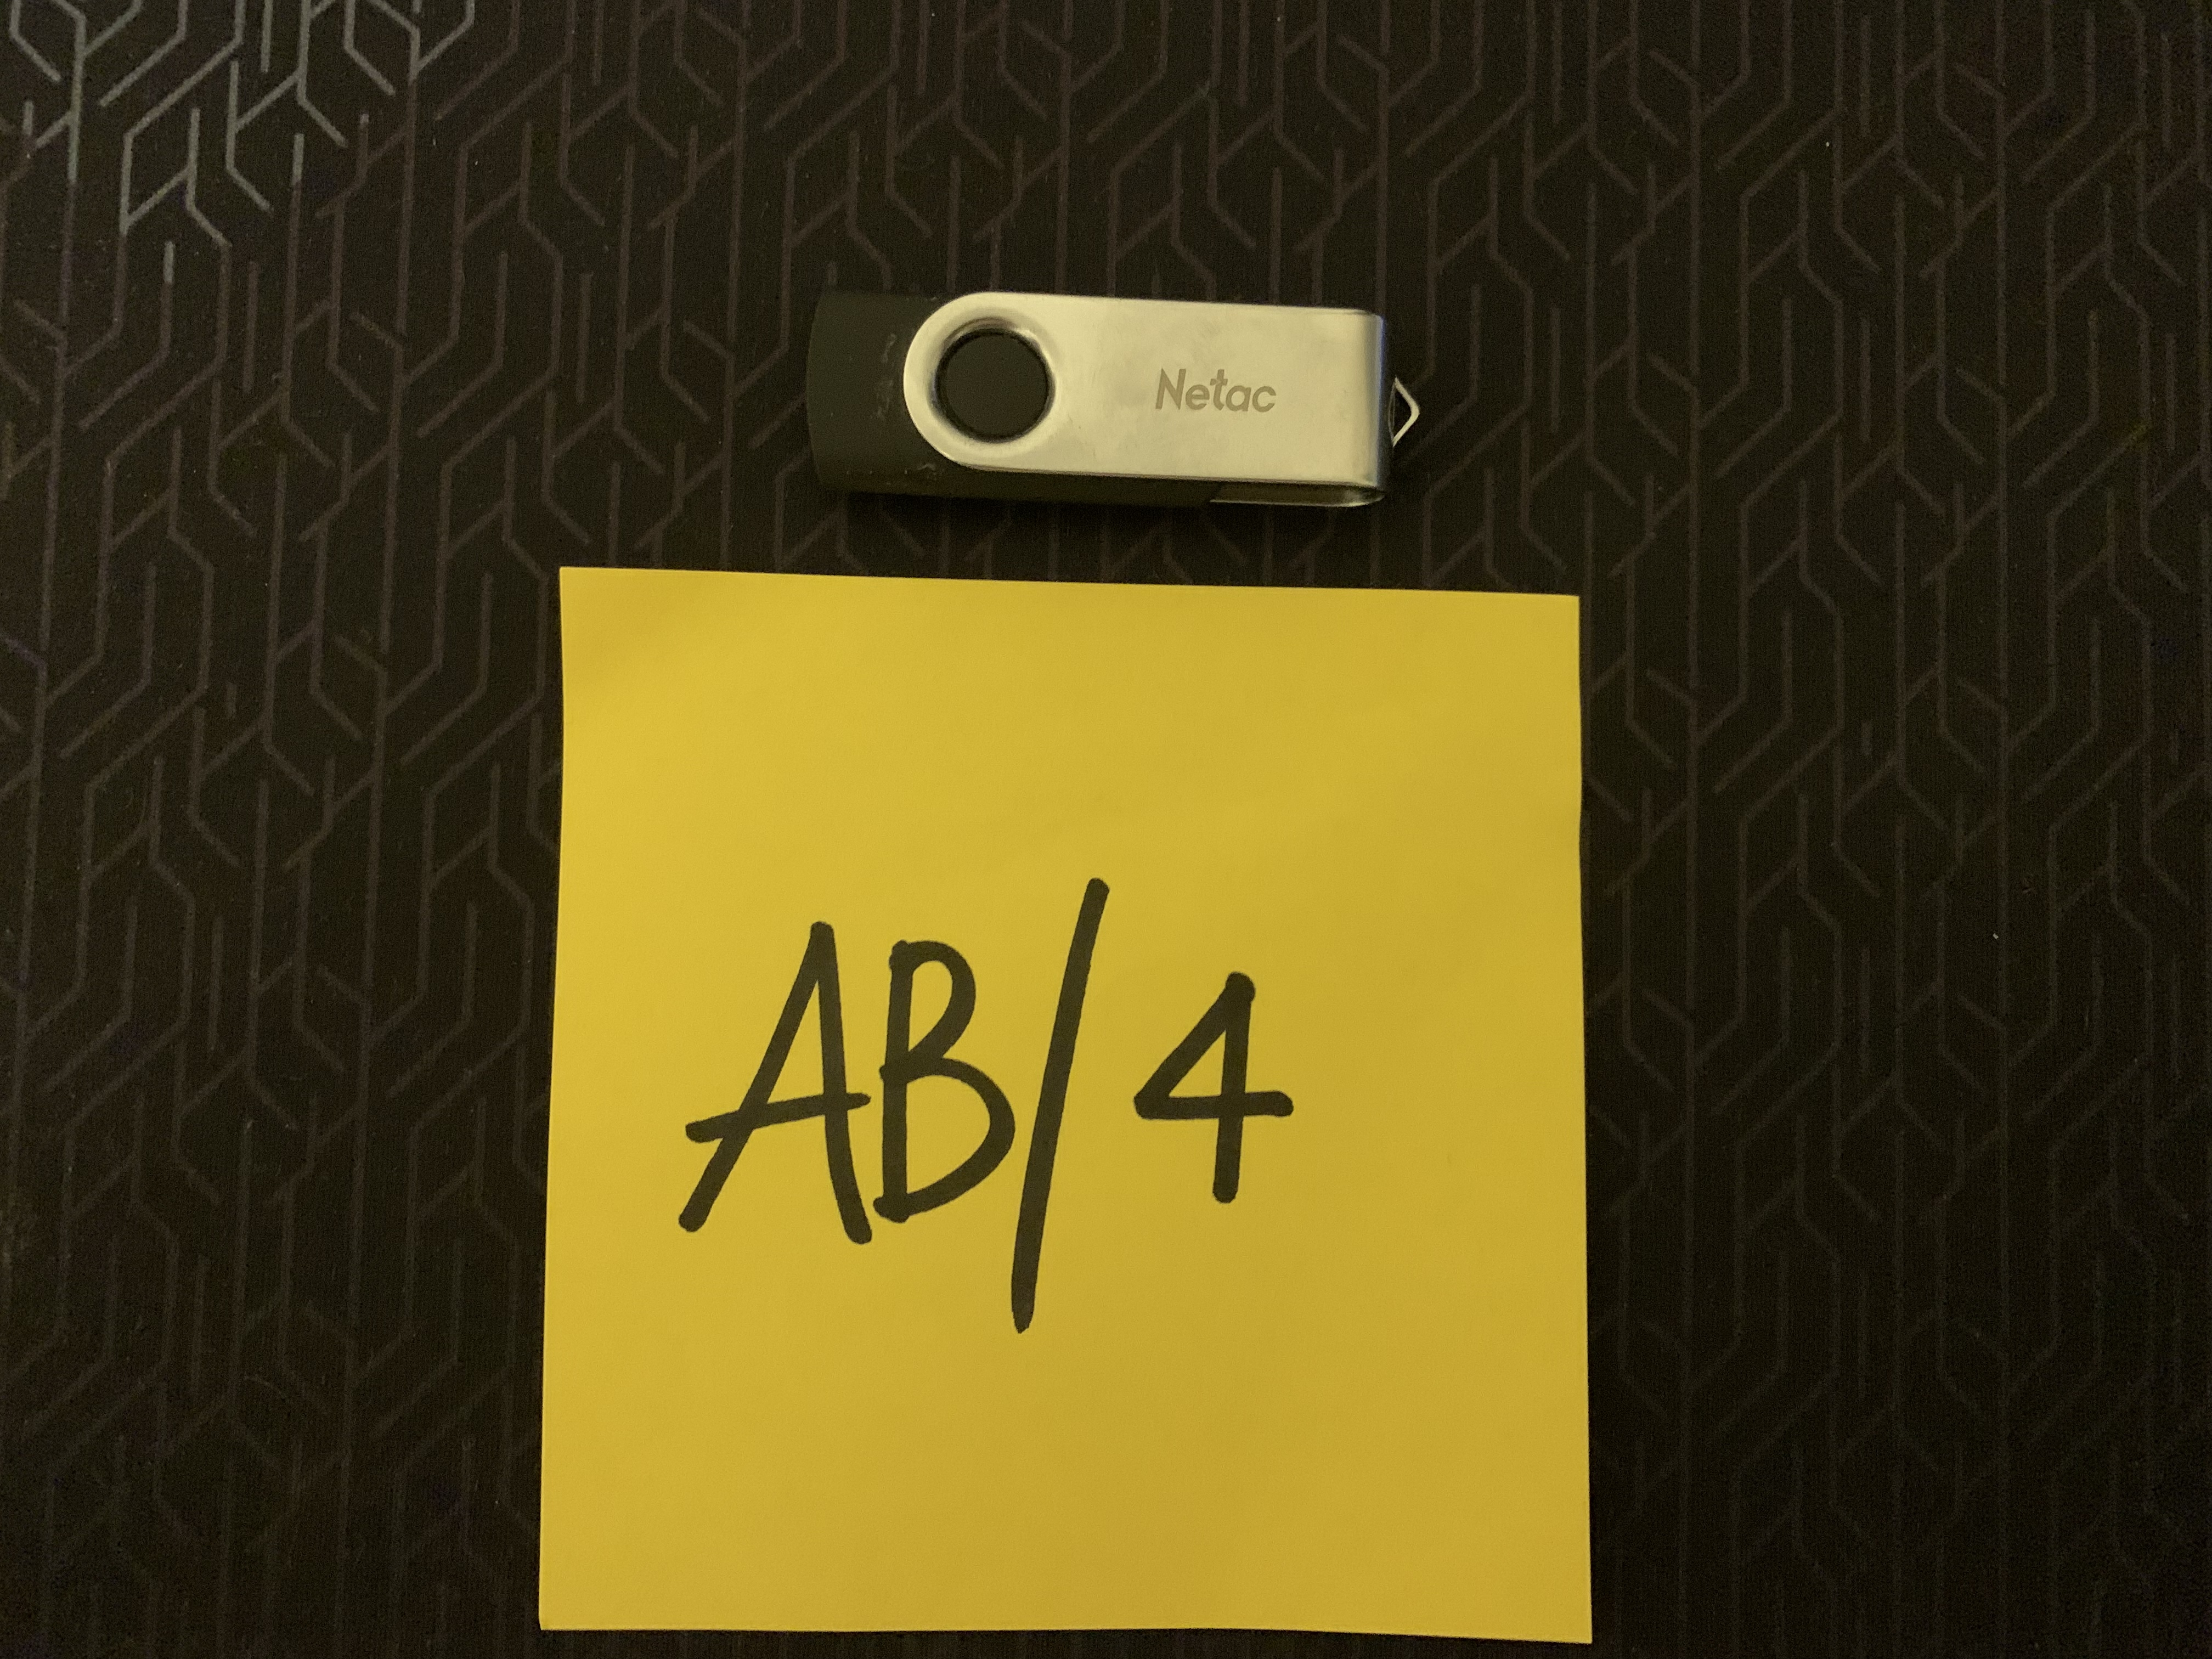
\includegraphics[width=0.7\textwidth]{figures/pictures/IMG_5049.JPG}
  \caption{Portable USB: Front}
  \label{fig:usb-front}
\end{figure}

\begin{figure}[h]
  \centering
  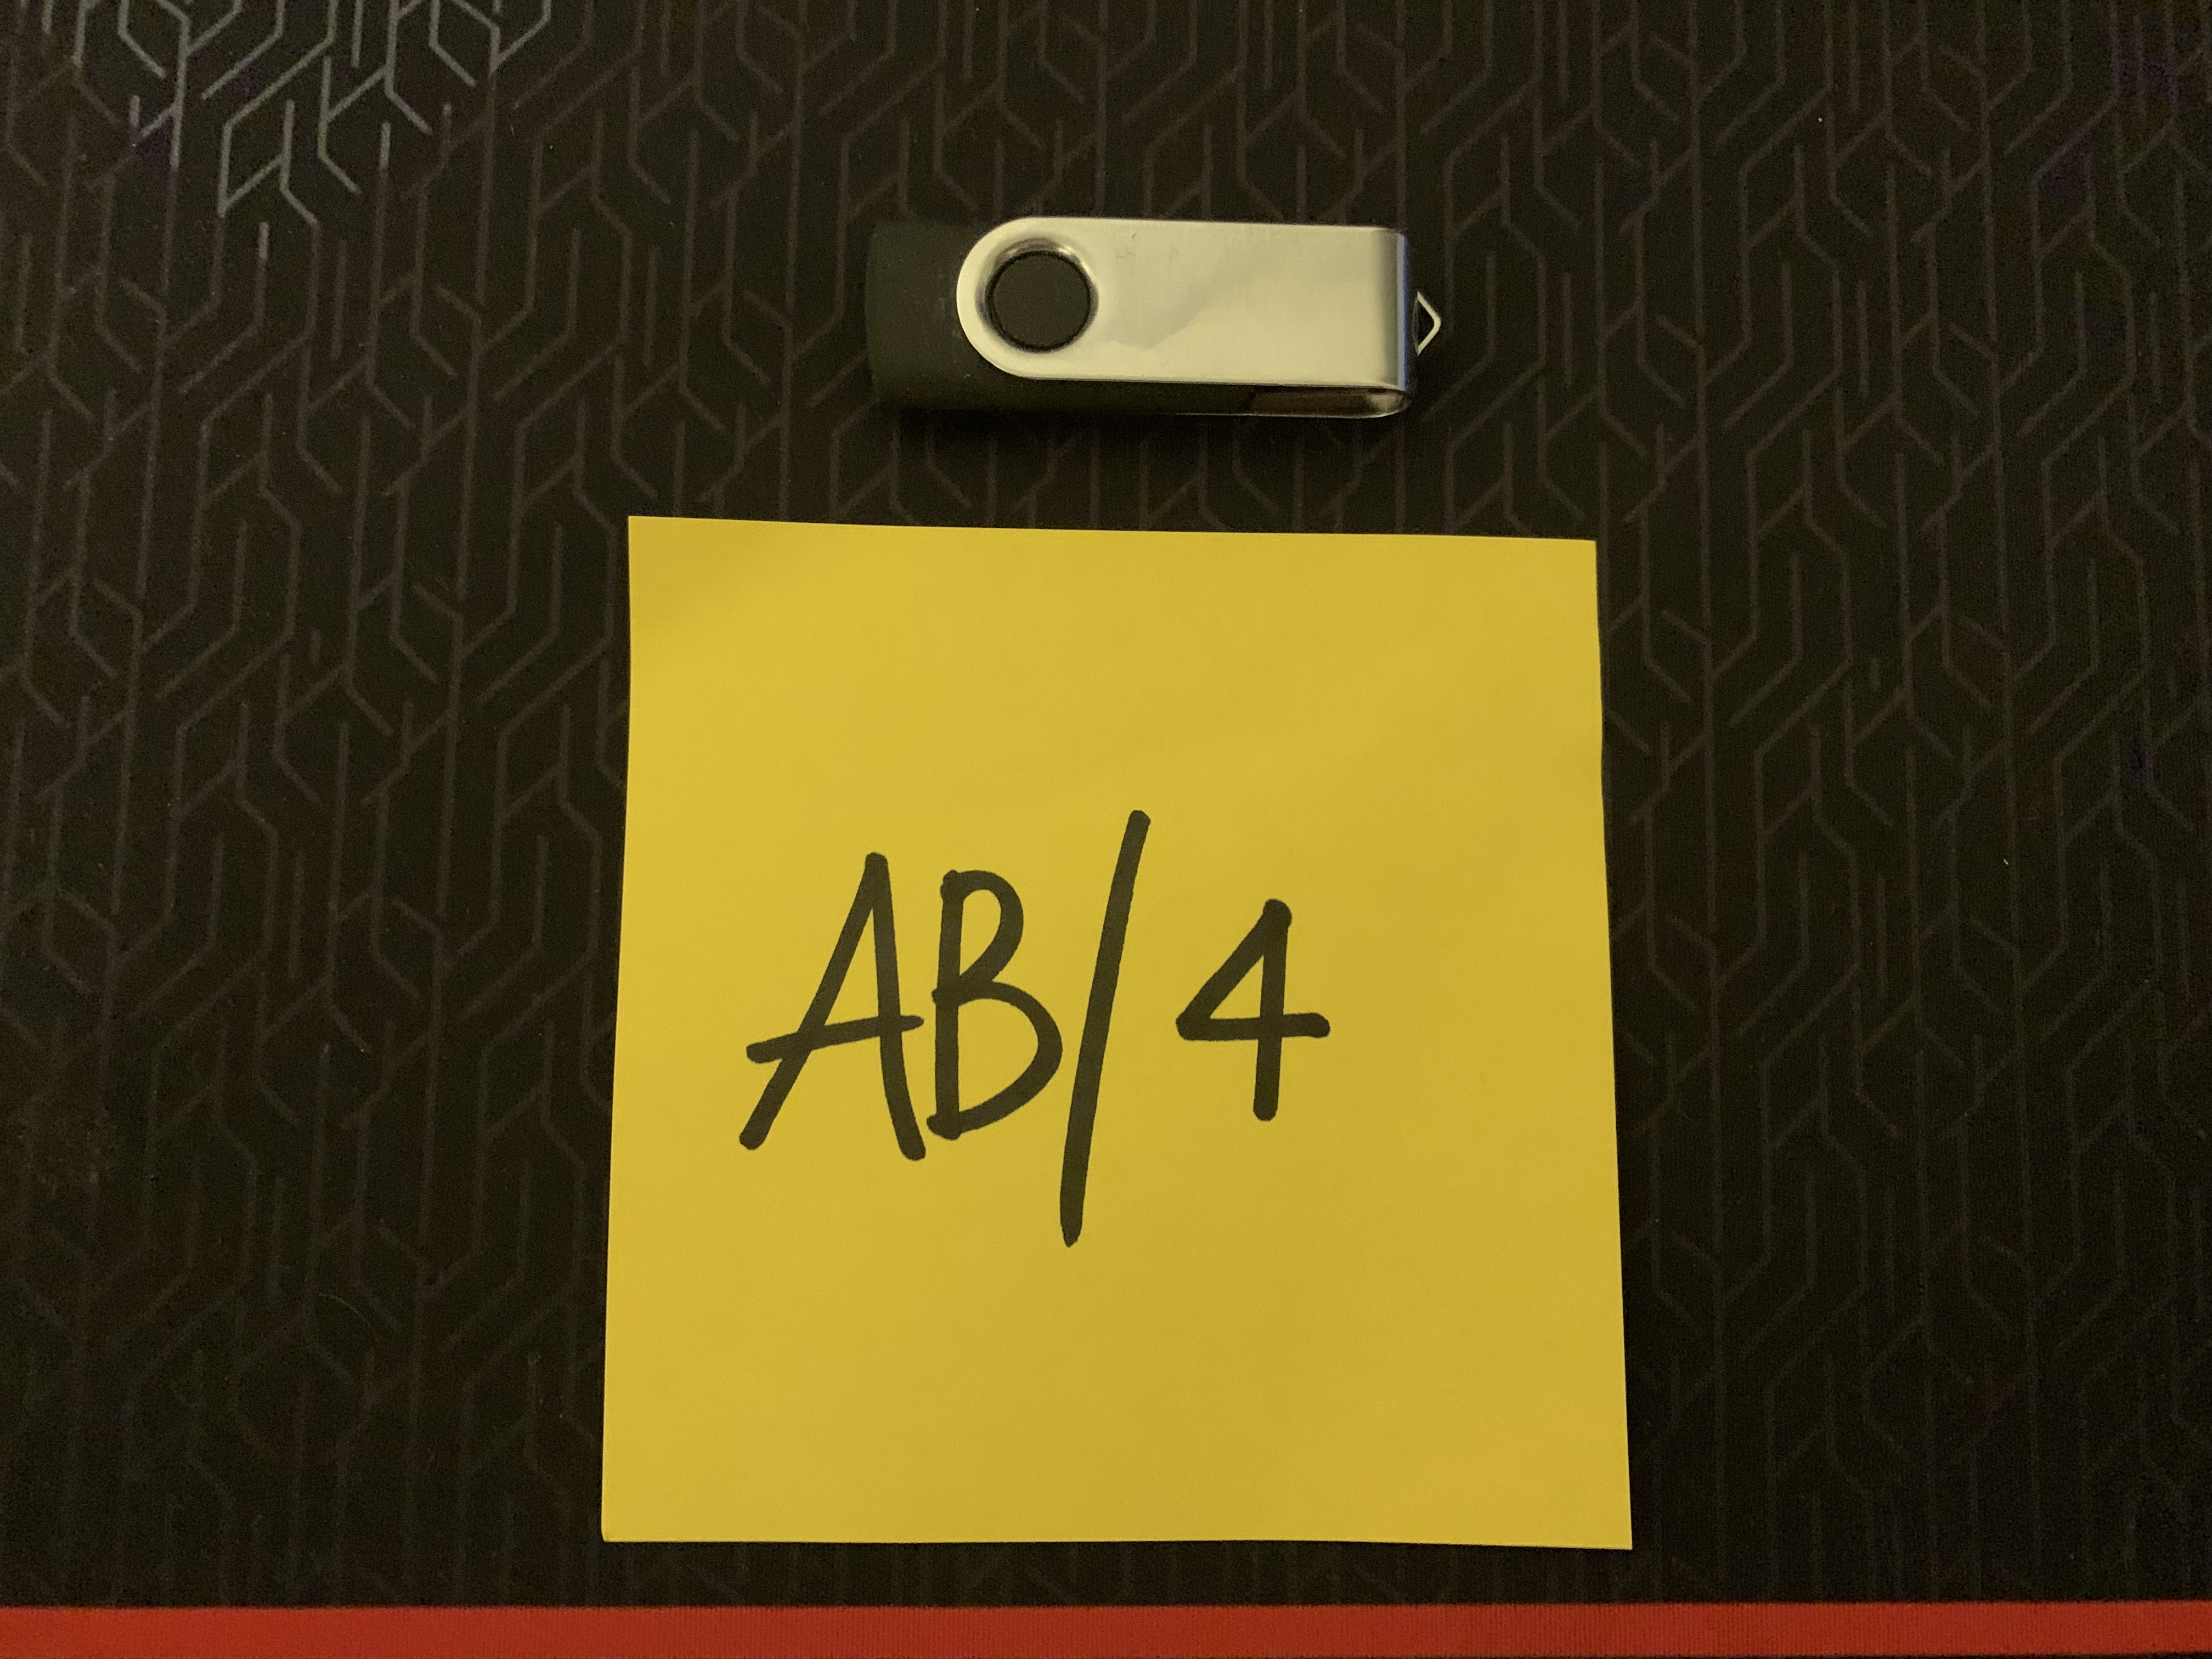
\includegraphics[width=0.7\textwidth]{figures/pictures/IMG_5050.JPG}
  \caption{Portable USB: Back}
  \label{fig:usb-back}
\end{figure}
\newpage

\subsection{Exhibit AB/5 (Apple Watch)}
\label{s:ab5}

\begin{figure}[h]
  \centering
  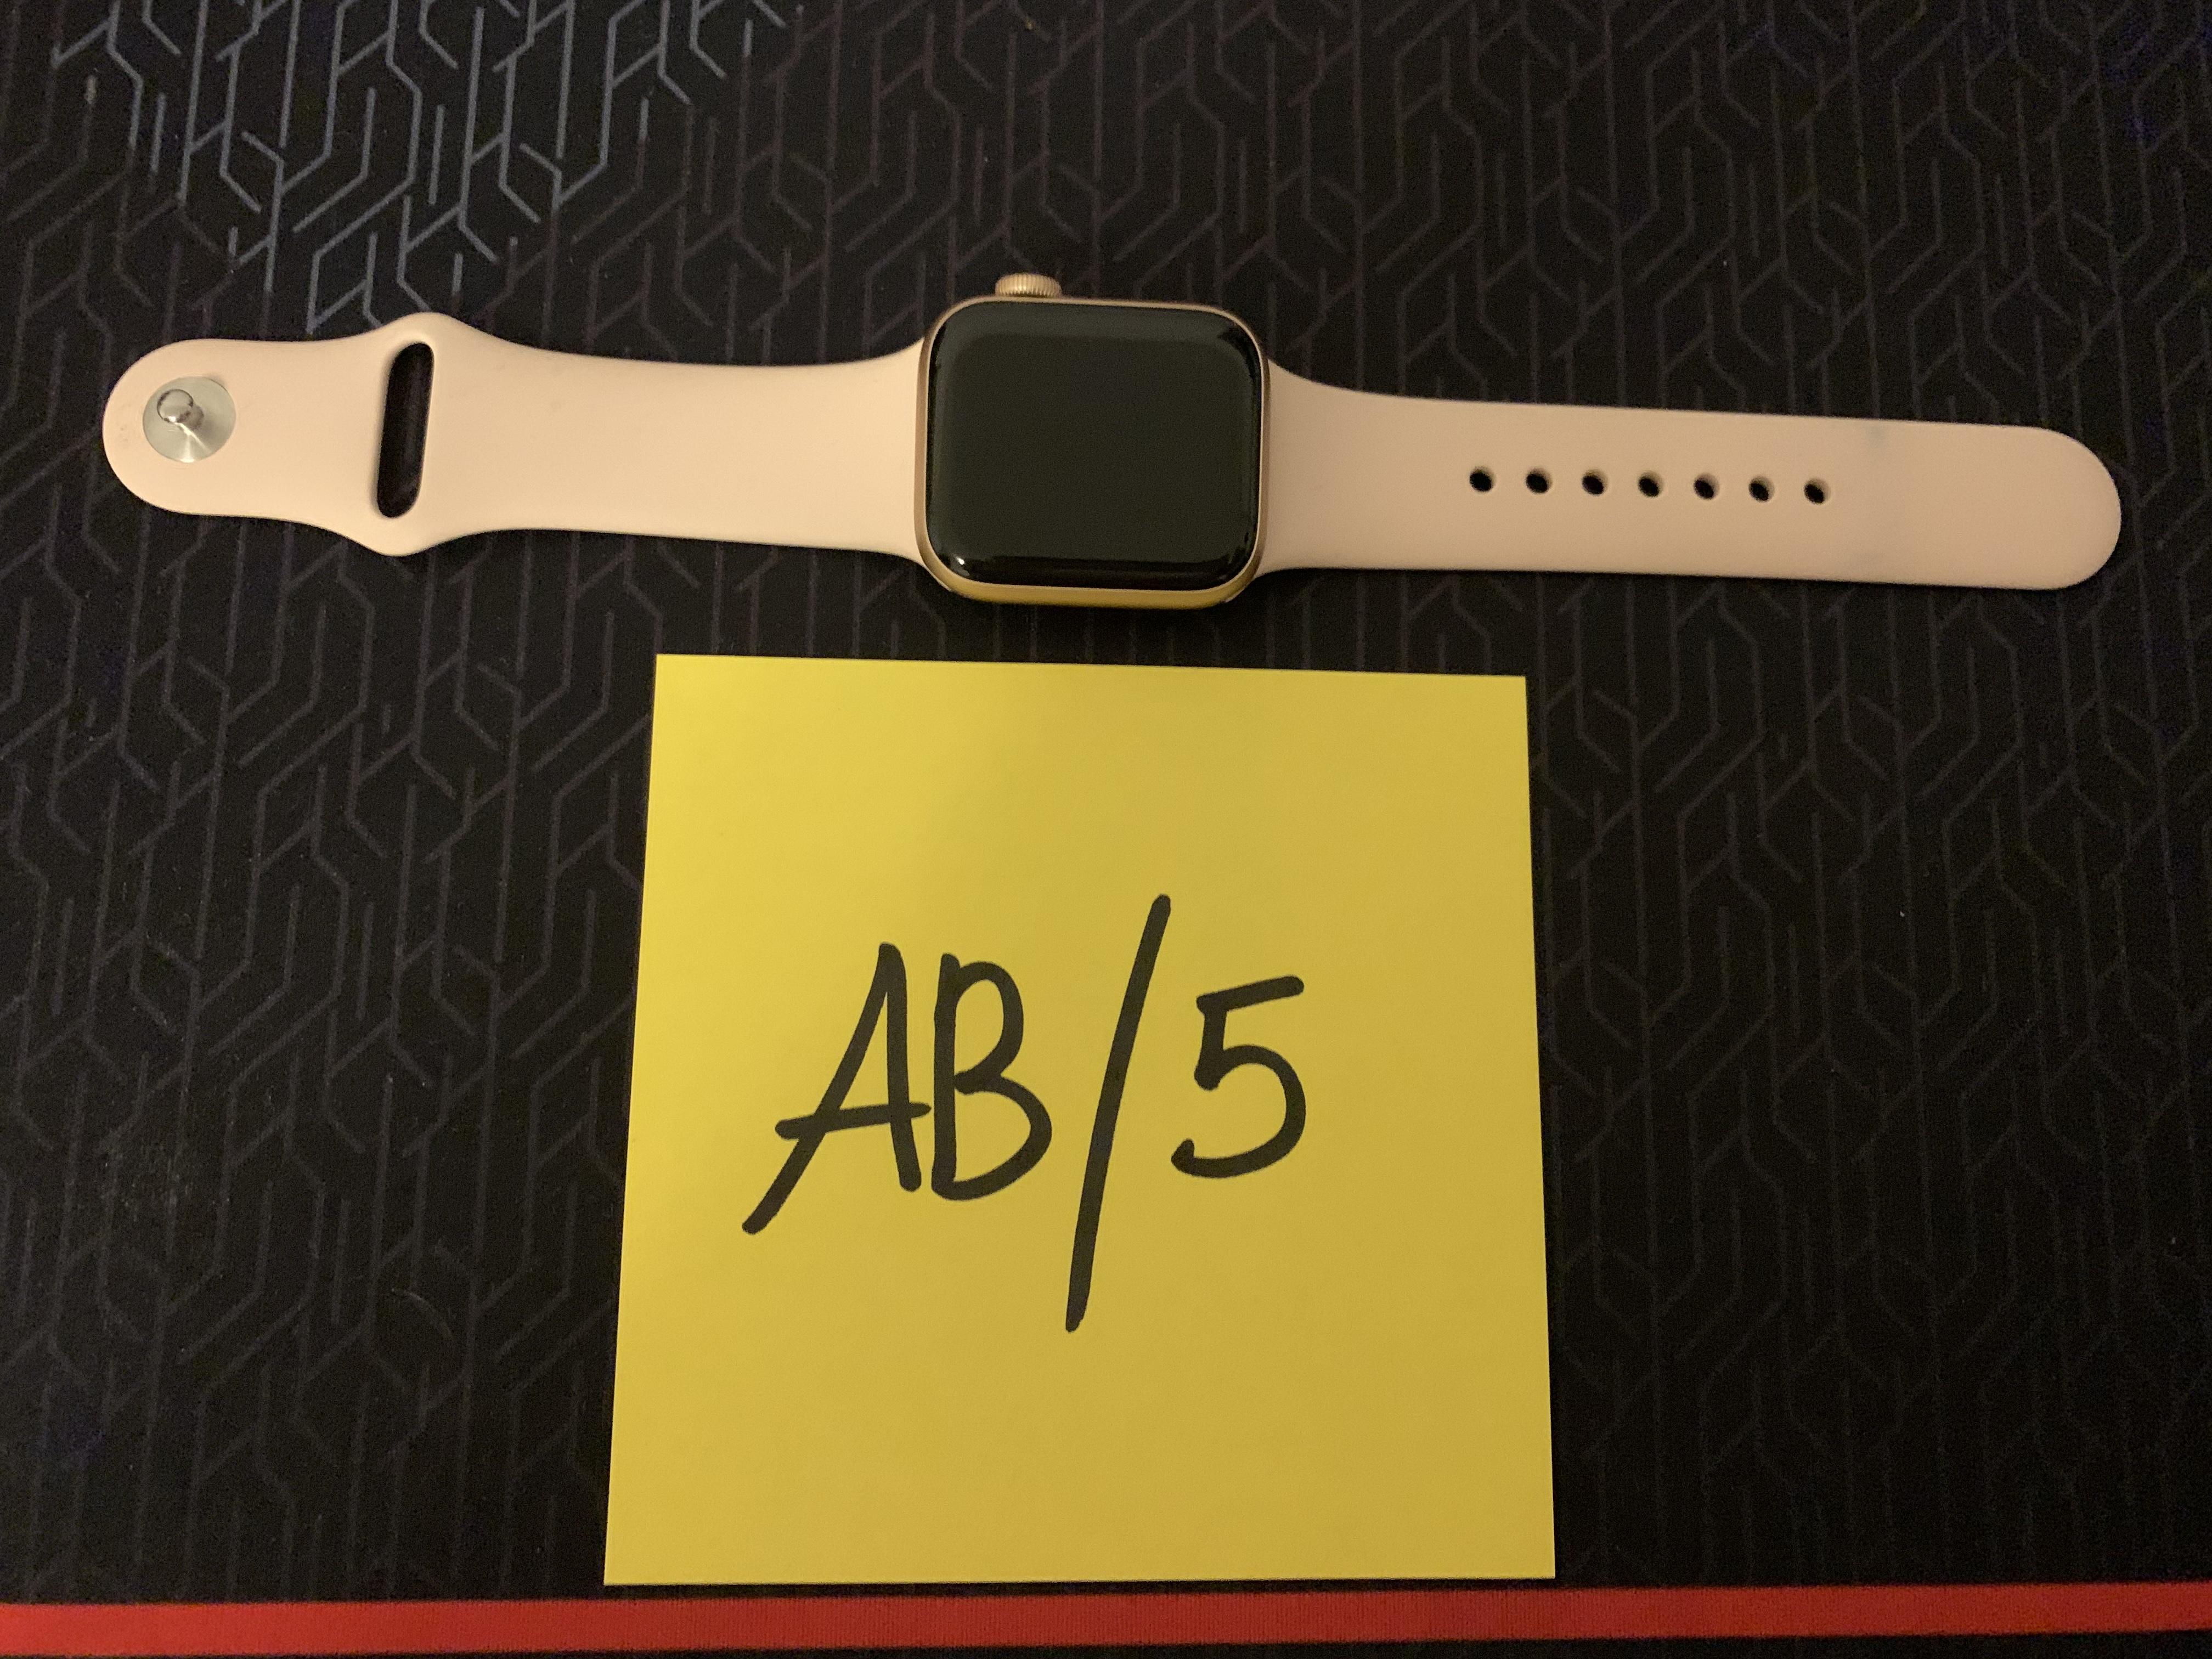
\includegraphics[width=0.7\textwidth]{figures/pictures/IMG_5051.JPG}
  \caption{Apple Watch: Front}
  \label{fig:watch-front}
\end{figure}

\begin{figure}[h]
  \centering
  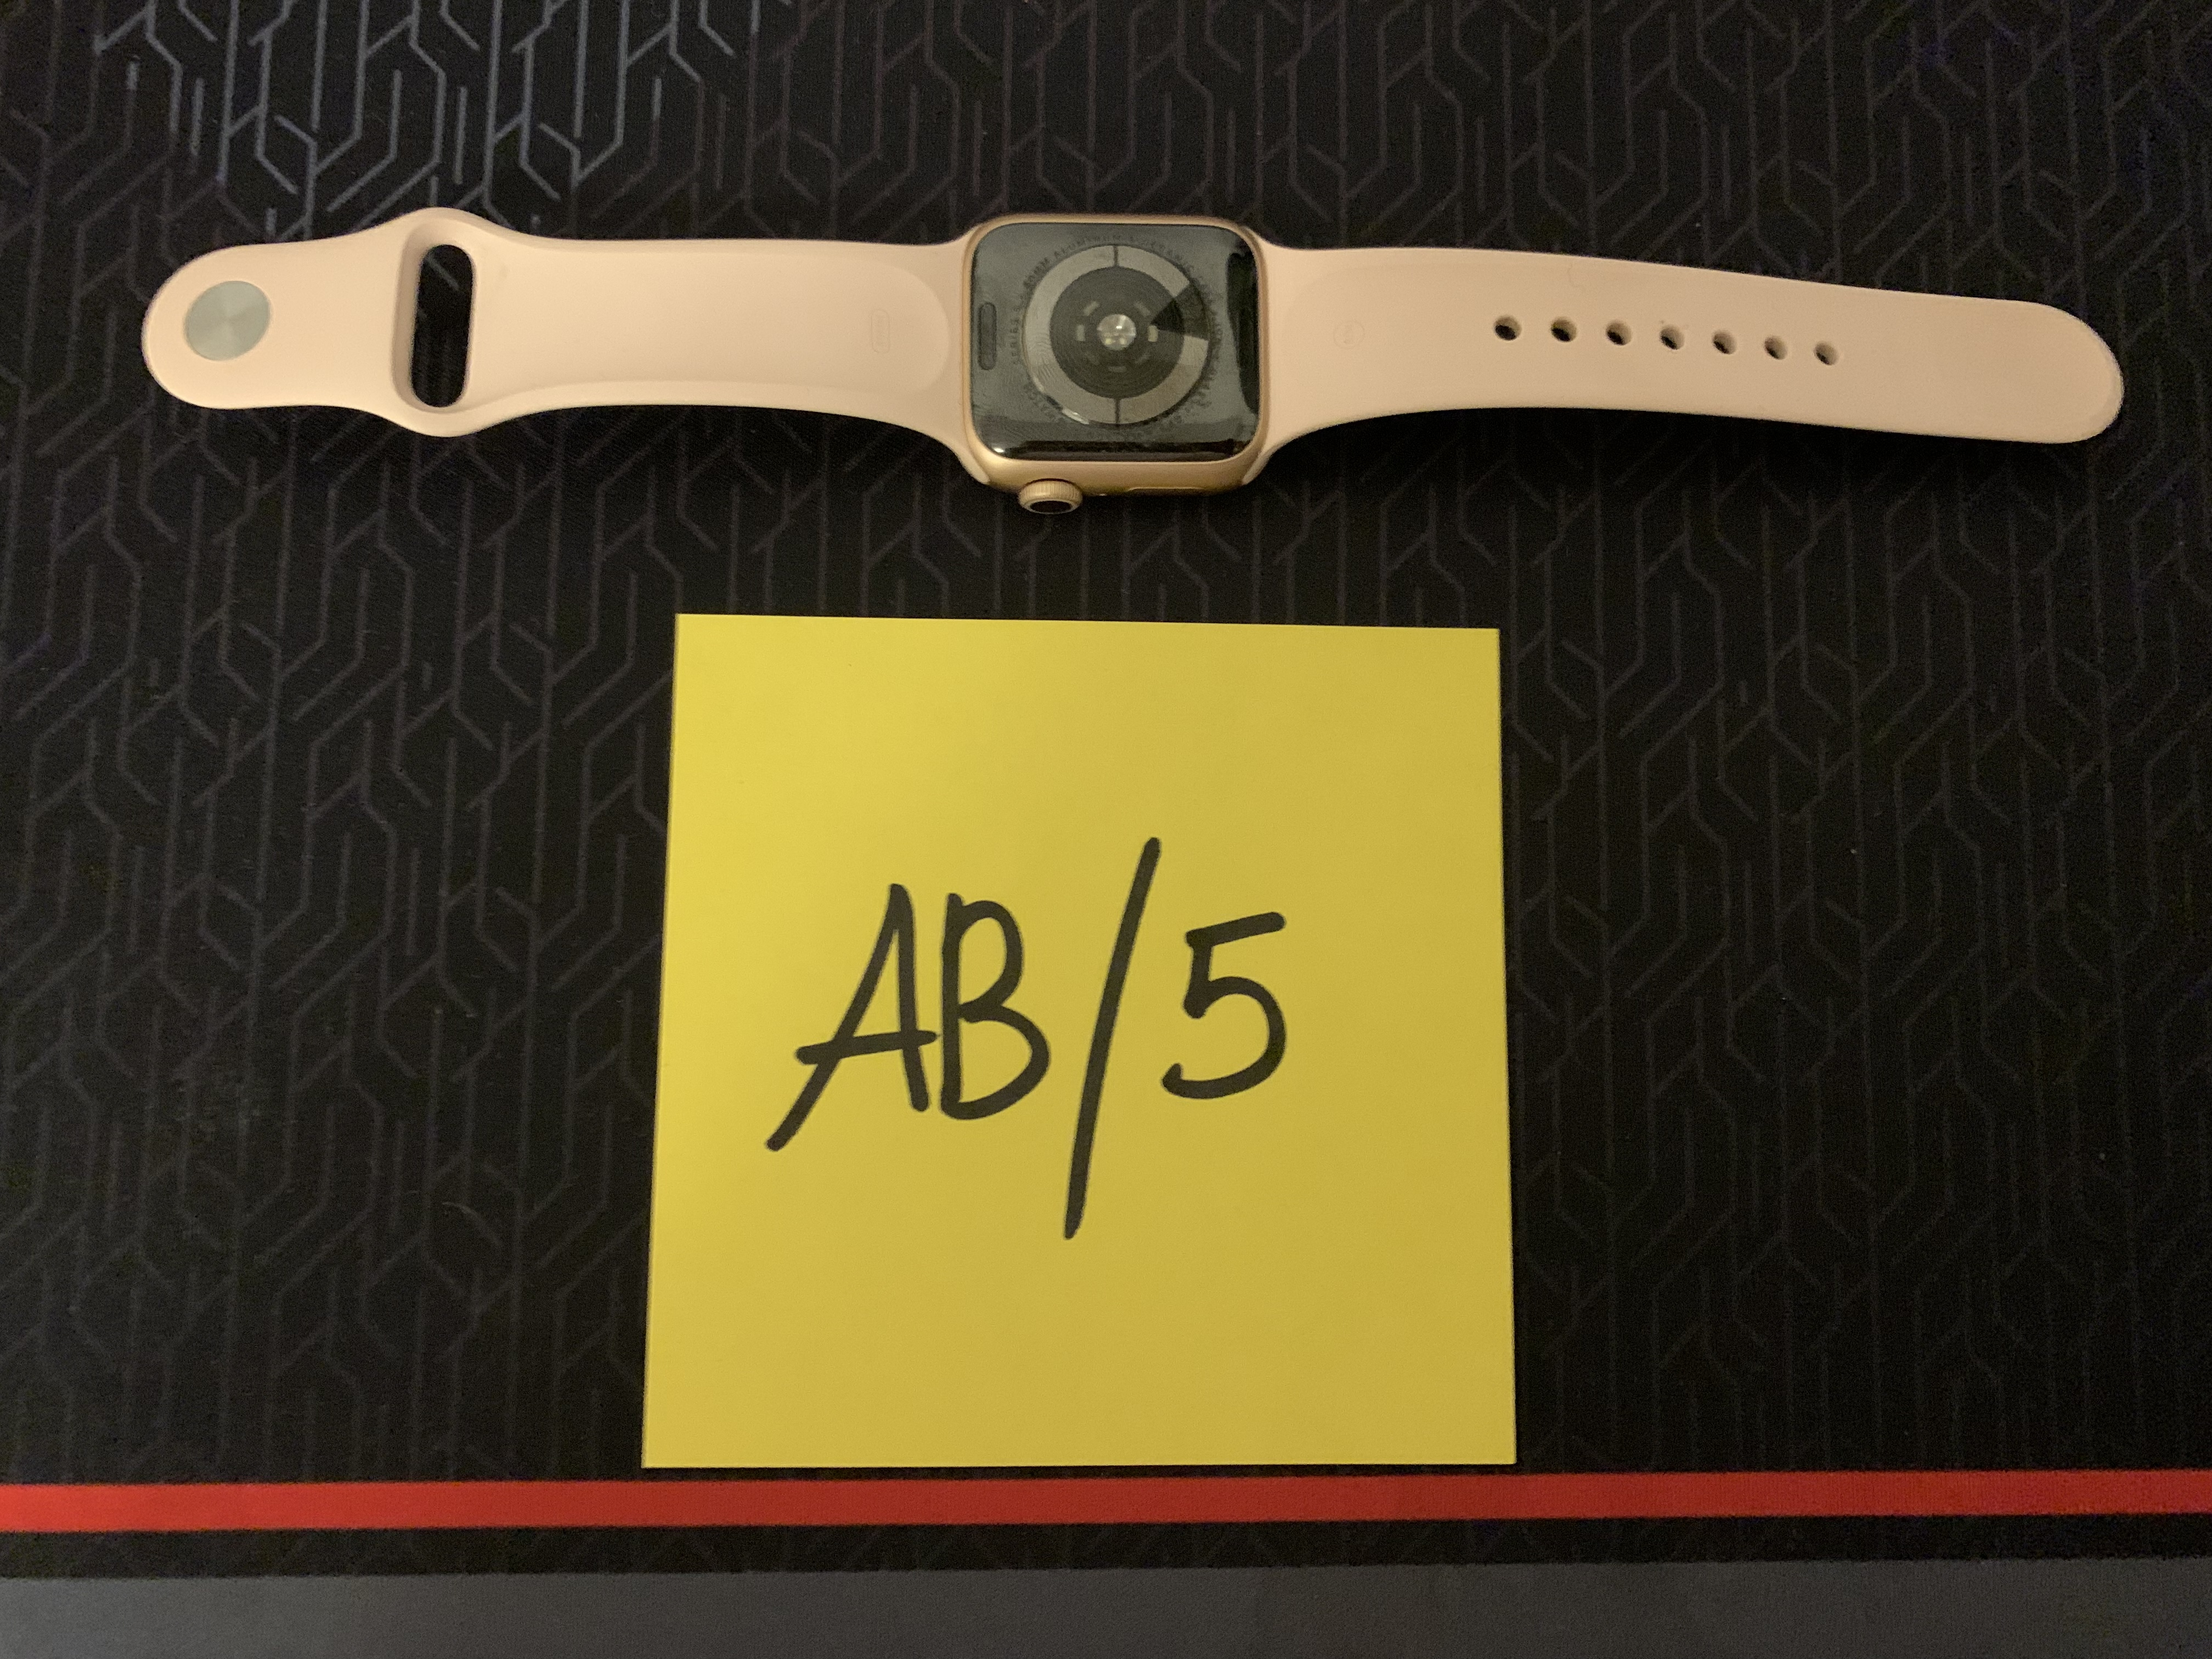
\includegraphics[width=0.7\textwidth]{figures/pictures/IMG_5052.JPG}
  \caption{Apple Watch: Back}
  \label{fig:watch-back}
\end{figure}
\newpage

\section{Exhibit Records}
\label{s:exhibit-records}

\subsection{AB/1: Laptop}
\label{s:ab1-laptop}
\begin{description}[align=left]
  \item [Location:] Right Desk
  \item [Seized by:] Alessandro Buonerba
  \item [Time:] 29/10/2021 at 16:00
\end{description}

\subsection{AB/2: HDD}
\label{s:ab2-hdd}
\begin{description}[align=left]
  \item [Location:] Right Desk
  \item [Seized by:] Alessandro Buonerba
  \item [Time:] 29/10/2021 at 16:10
\end{description}

\subsection{AB/3: Smartphone}
\label{s:ab3-smartphone}
\begin{description}[align=left]
  \item [Location:] Right Desk
  \item [Seized by:] Alessandro Buonerba
  \item [Time:] 29/10/2021 at 16:15
\end{description}

\subsection{AB/4: Portable USB}
\label{s:ab4-usb}
\begin{description}[align=left]
  \item [Location:] Chest of drawer
  \item [Seized by:] Alessandro Buonerba
  \item [Time:] 29/10/2021 at 16:25
  \item [Seal Number]: AB
\end{description}

\subsection{AB/5: Apple Watch}
\label{s:ab5-watch}
\begin{description}[align=left]
  \item [Location:] Left Desk
  \item [Seized by:] Alessandro Buonerba
  \item [Time:] 29/10/2021 at 16:40
\end{description}

\section{Sealed Evidences}
\label{s:sealed-evidences}
The evidence that have been sealed is Exhibit AB/4 (\ref{s:ab4}). They have been
stored in a sealed envelope that cannot be tempered without leaving tracks of it.
If the seal breaks, there would be noticeable traces of it as shown in figure
\ref{fig:broken}.

\subsection{Sealed Exhibit AB/4 (Portable USB)}
\label{s:sealed-ab4}

\begin{figure}[h]
  \centering
  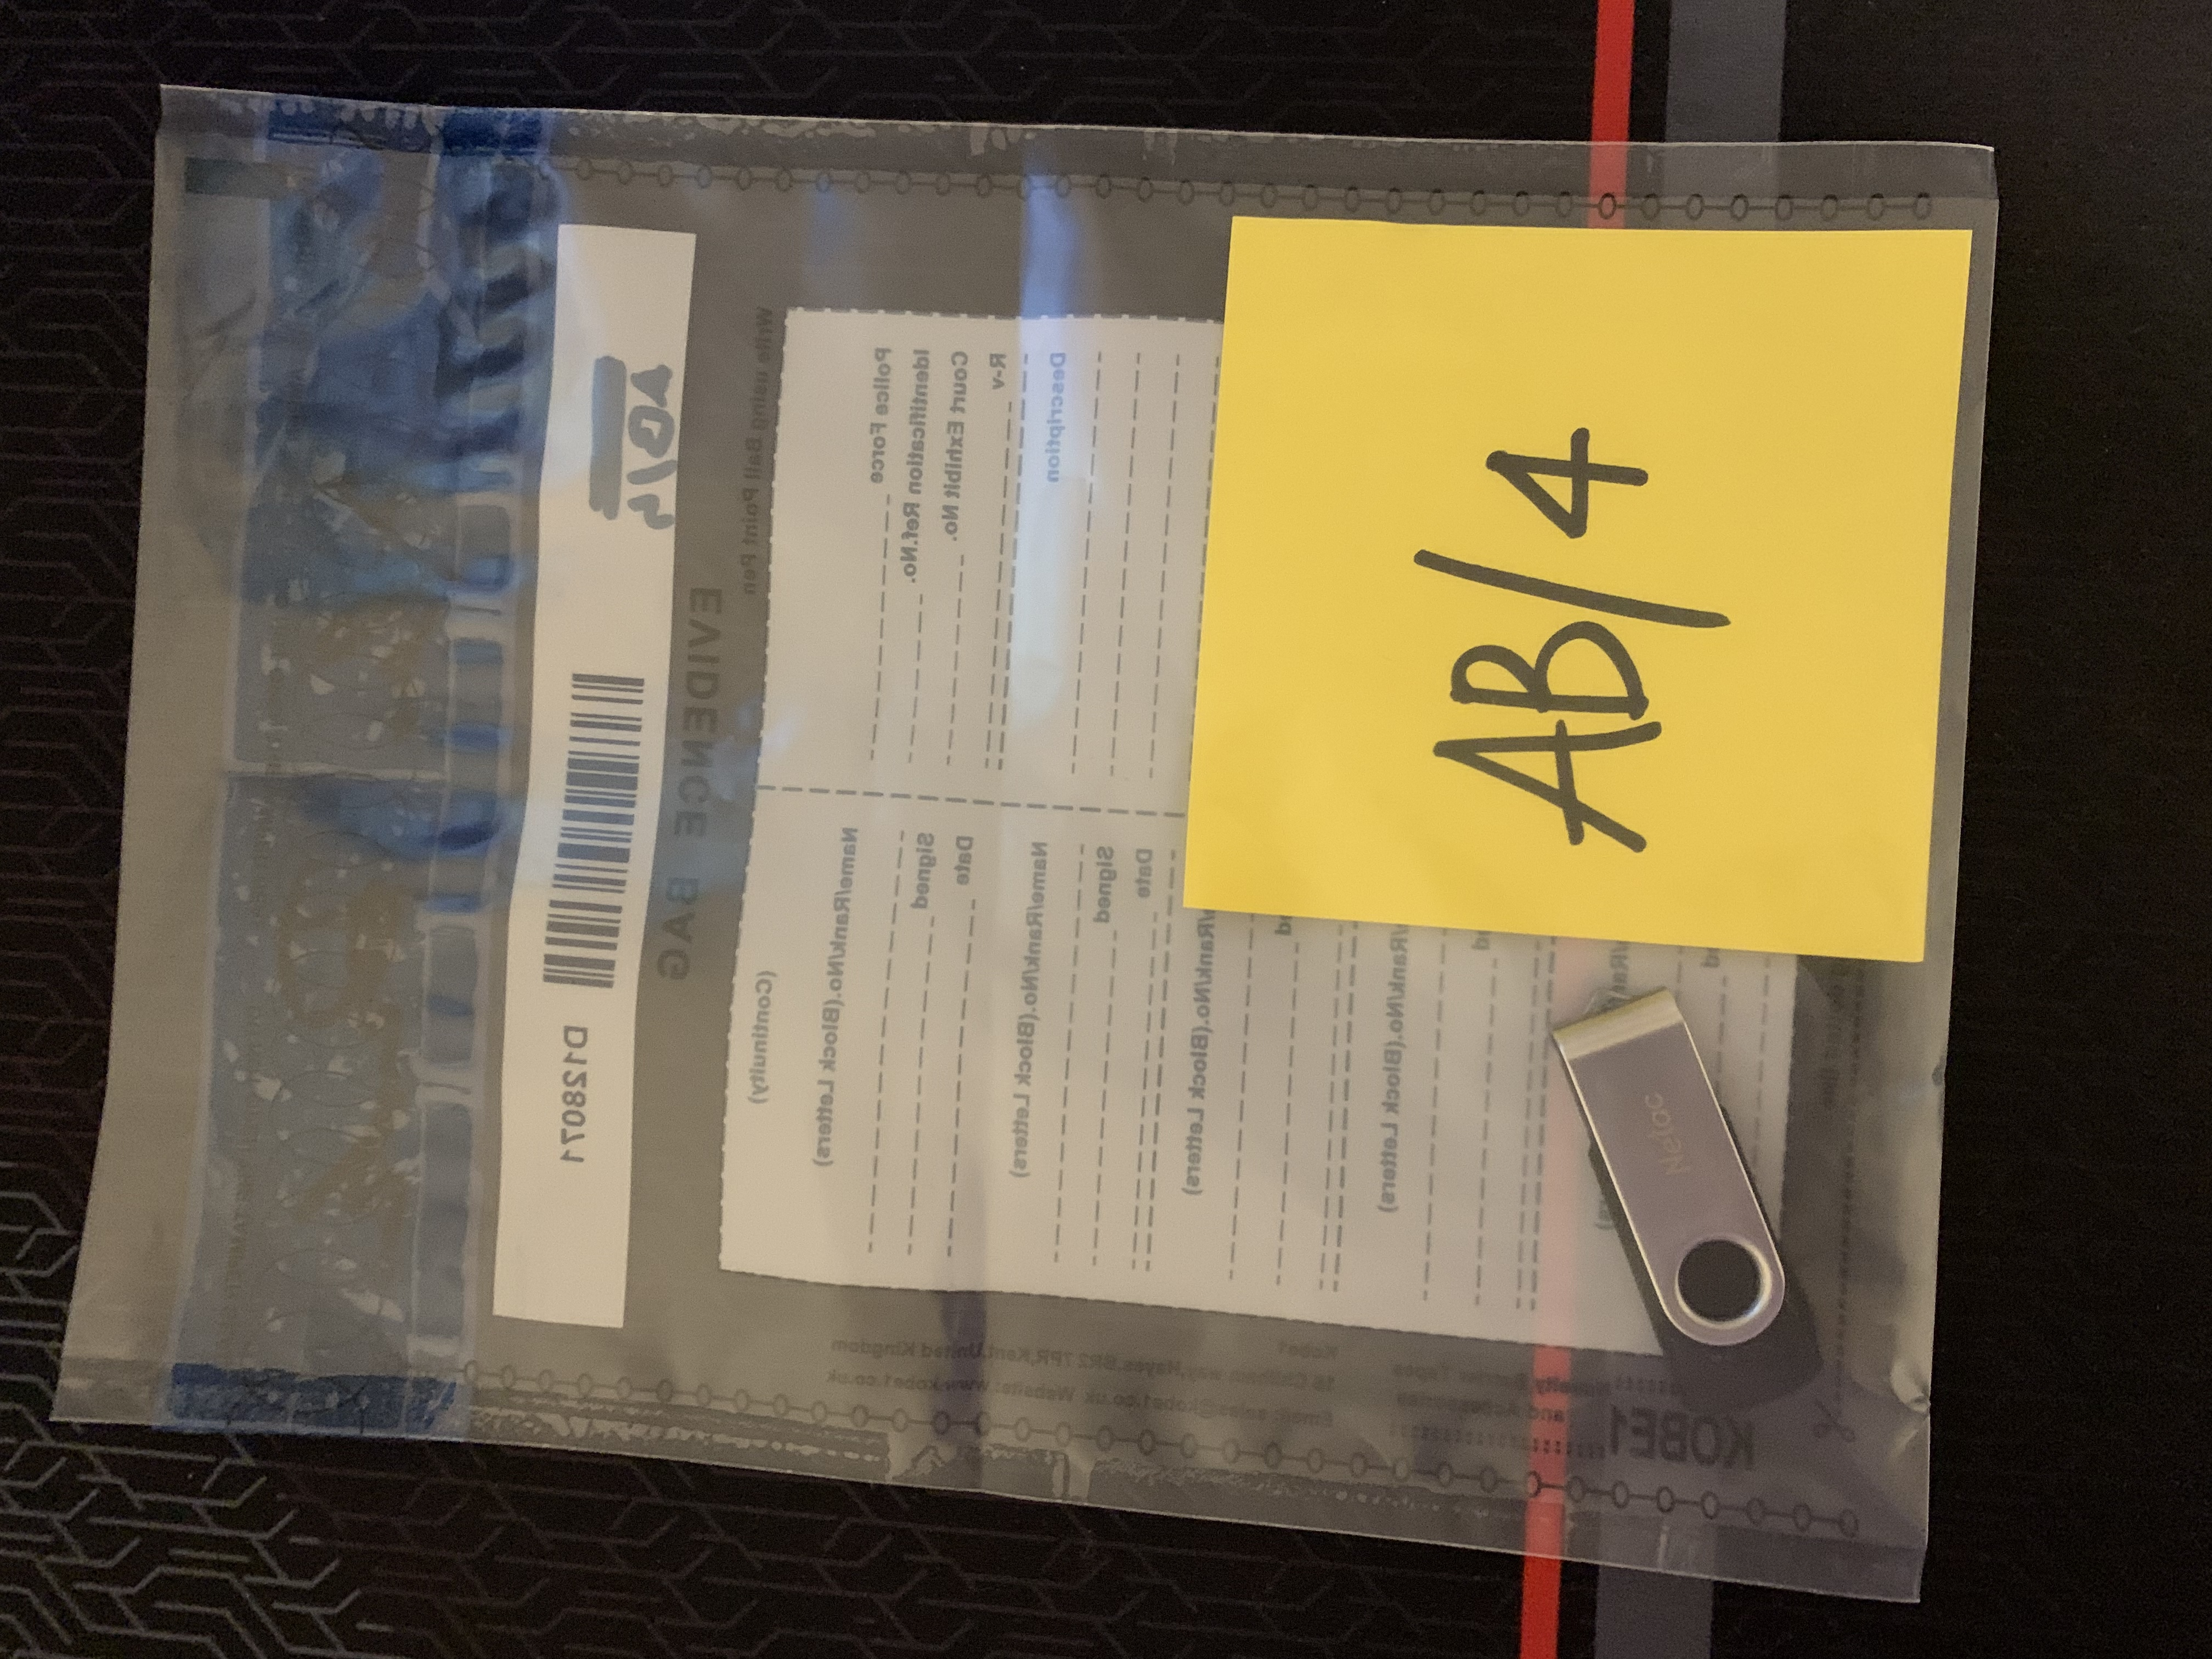
\includegraphics[width=0.55\textwidth, angle=-90,origin=c]{figures/pictures/IMG_5057.JPG}
  \caption{Sealed Portable USB: Back}
  \label{fig:sealed-usb-back}
\end{figure}

\begin{figure}[h]
  \centering
  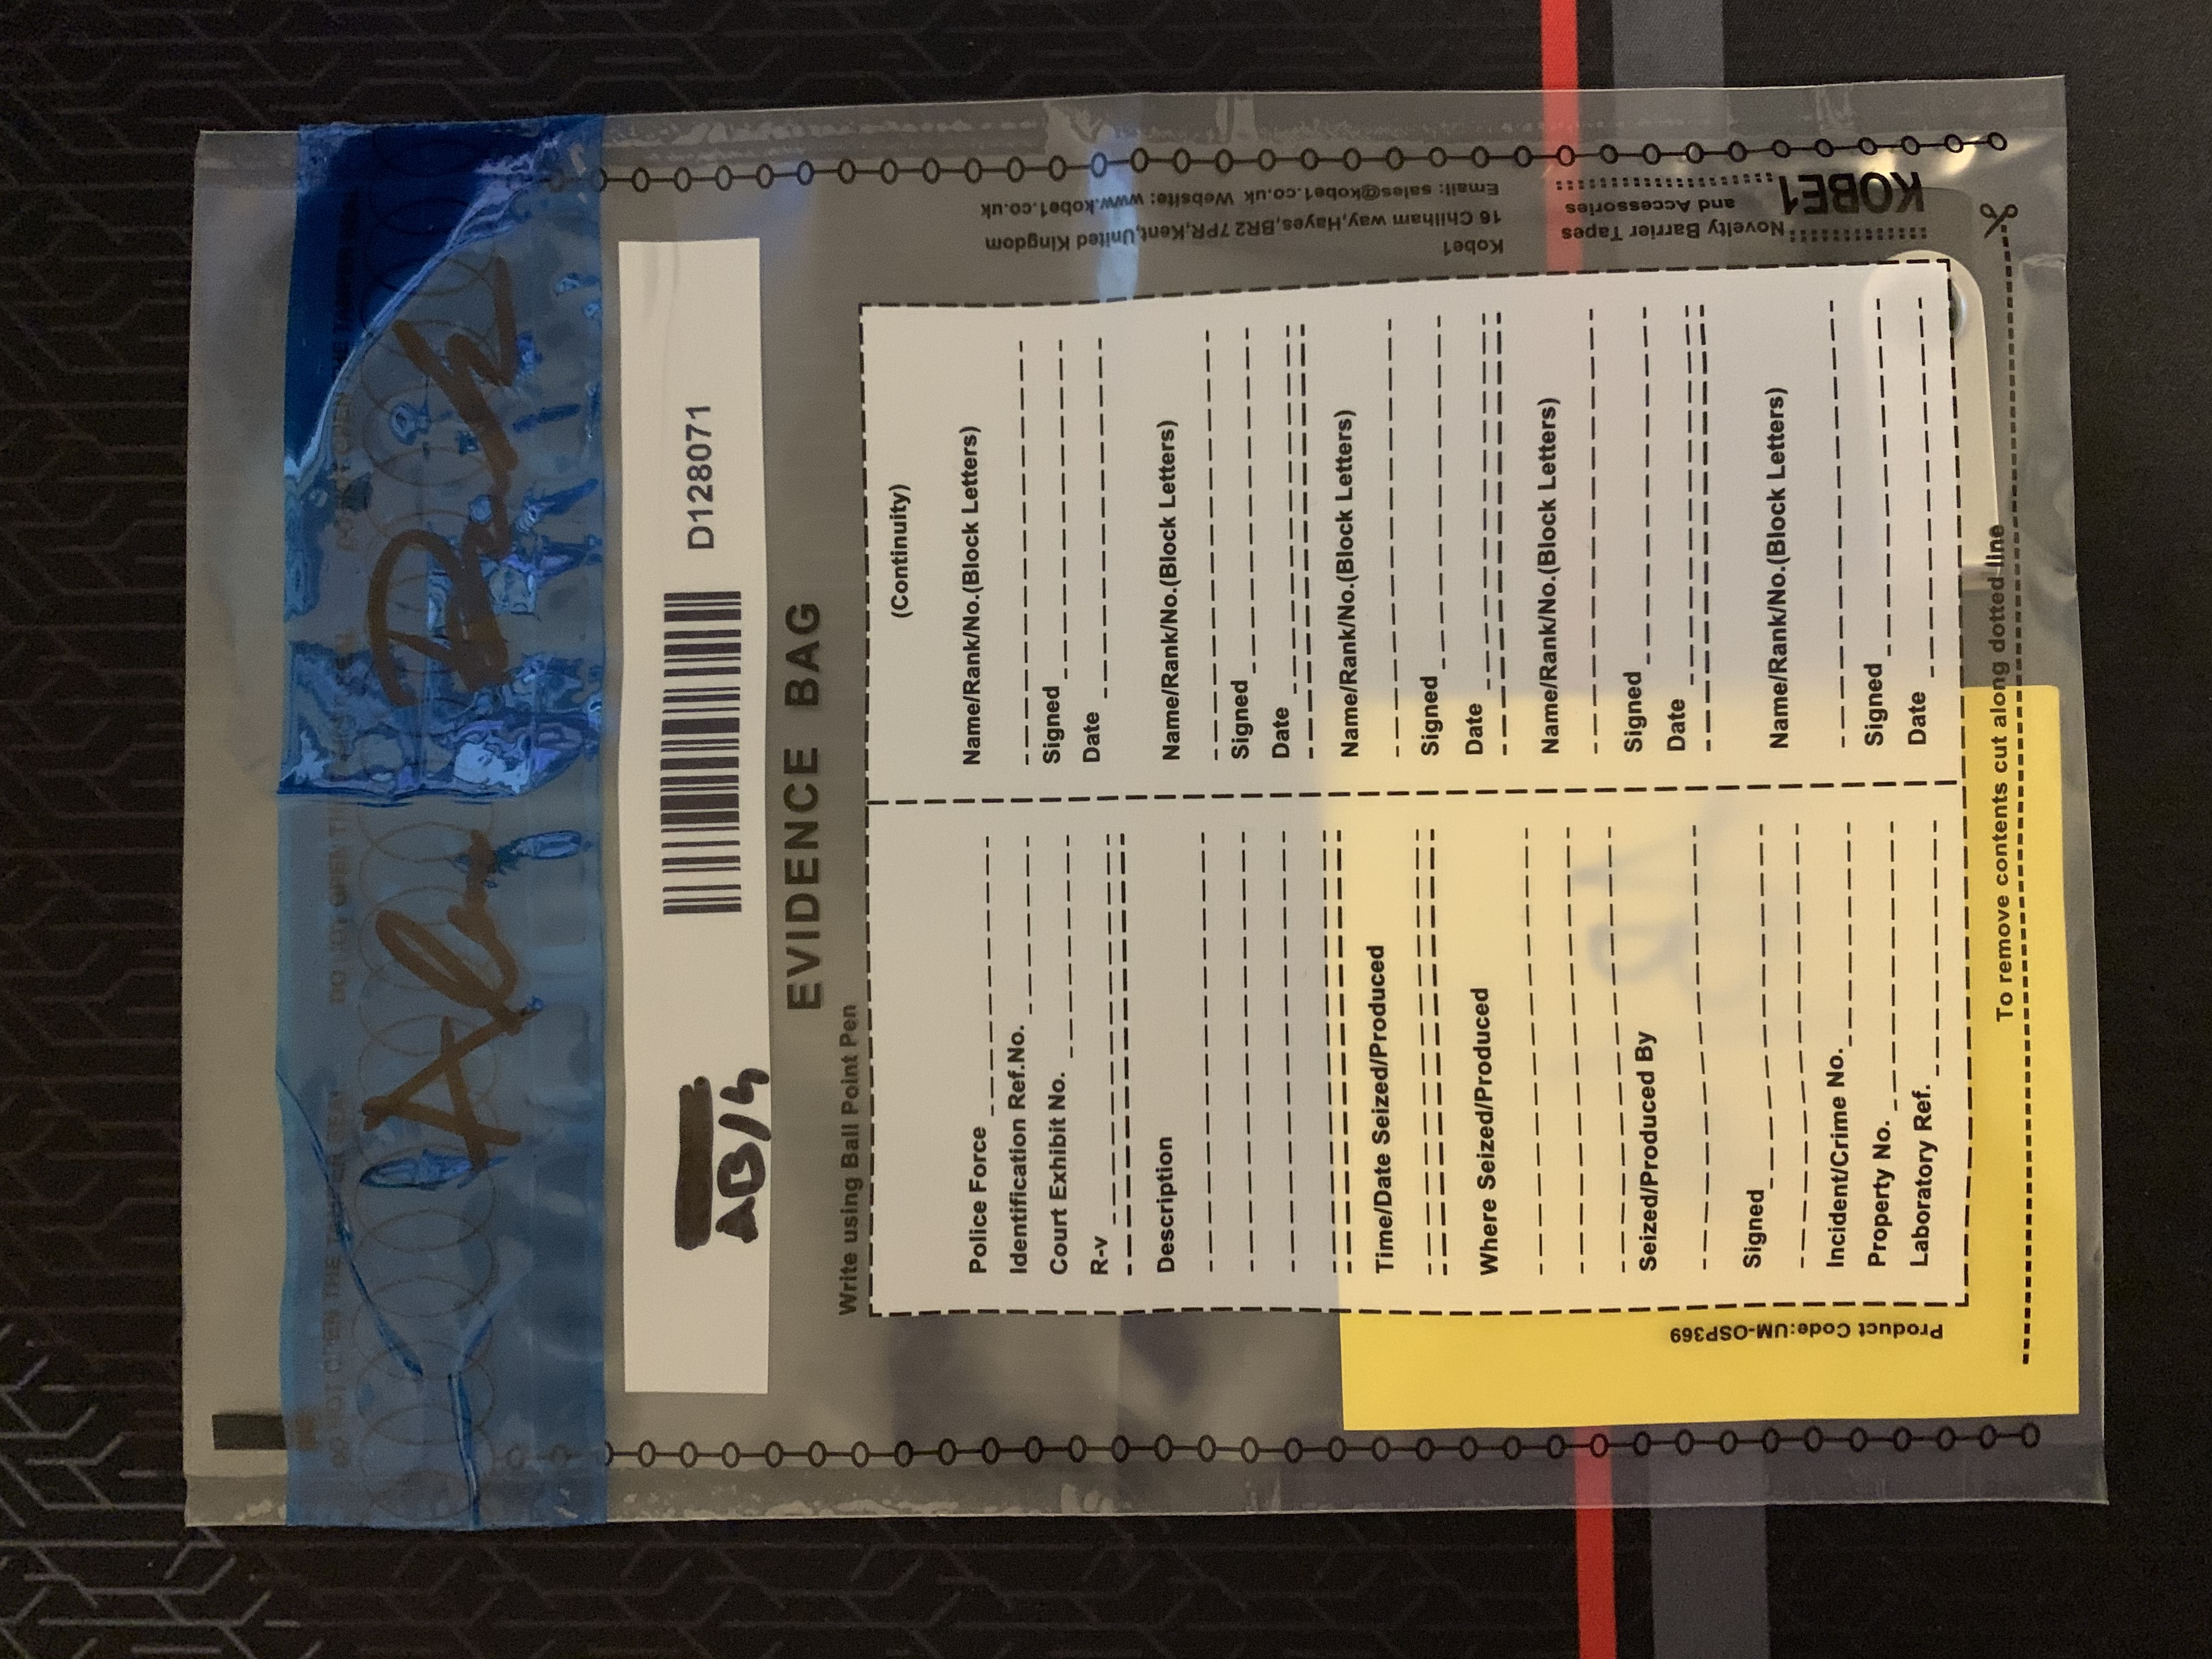
\includegraphics[width=0.55\textwidth, angle=-90,origin=c]{figures/pictures/IMG_5054.JPG}
  \caption{Sealed Portable USB: Front}
  \label{fig:sealed-usb-front}
\end{figure}
\newpage

\subsection{Seal}

Below a close-up of the seal is shown.
\label{s:closeup}
\begin{figure}[h]
  \centering
  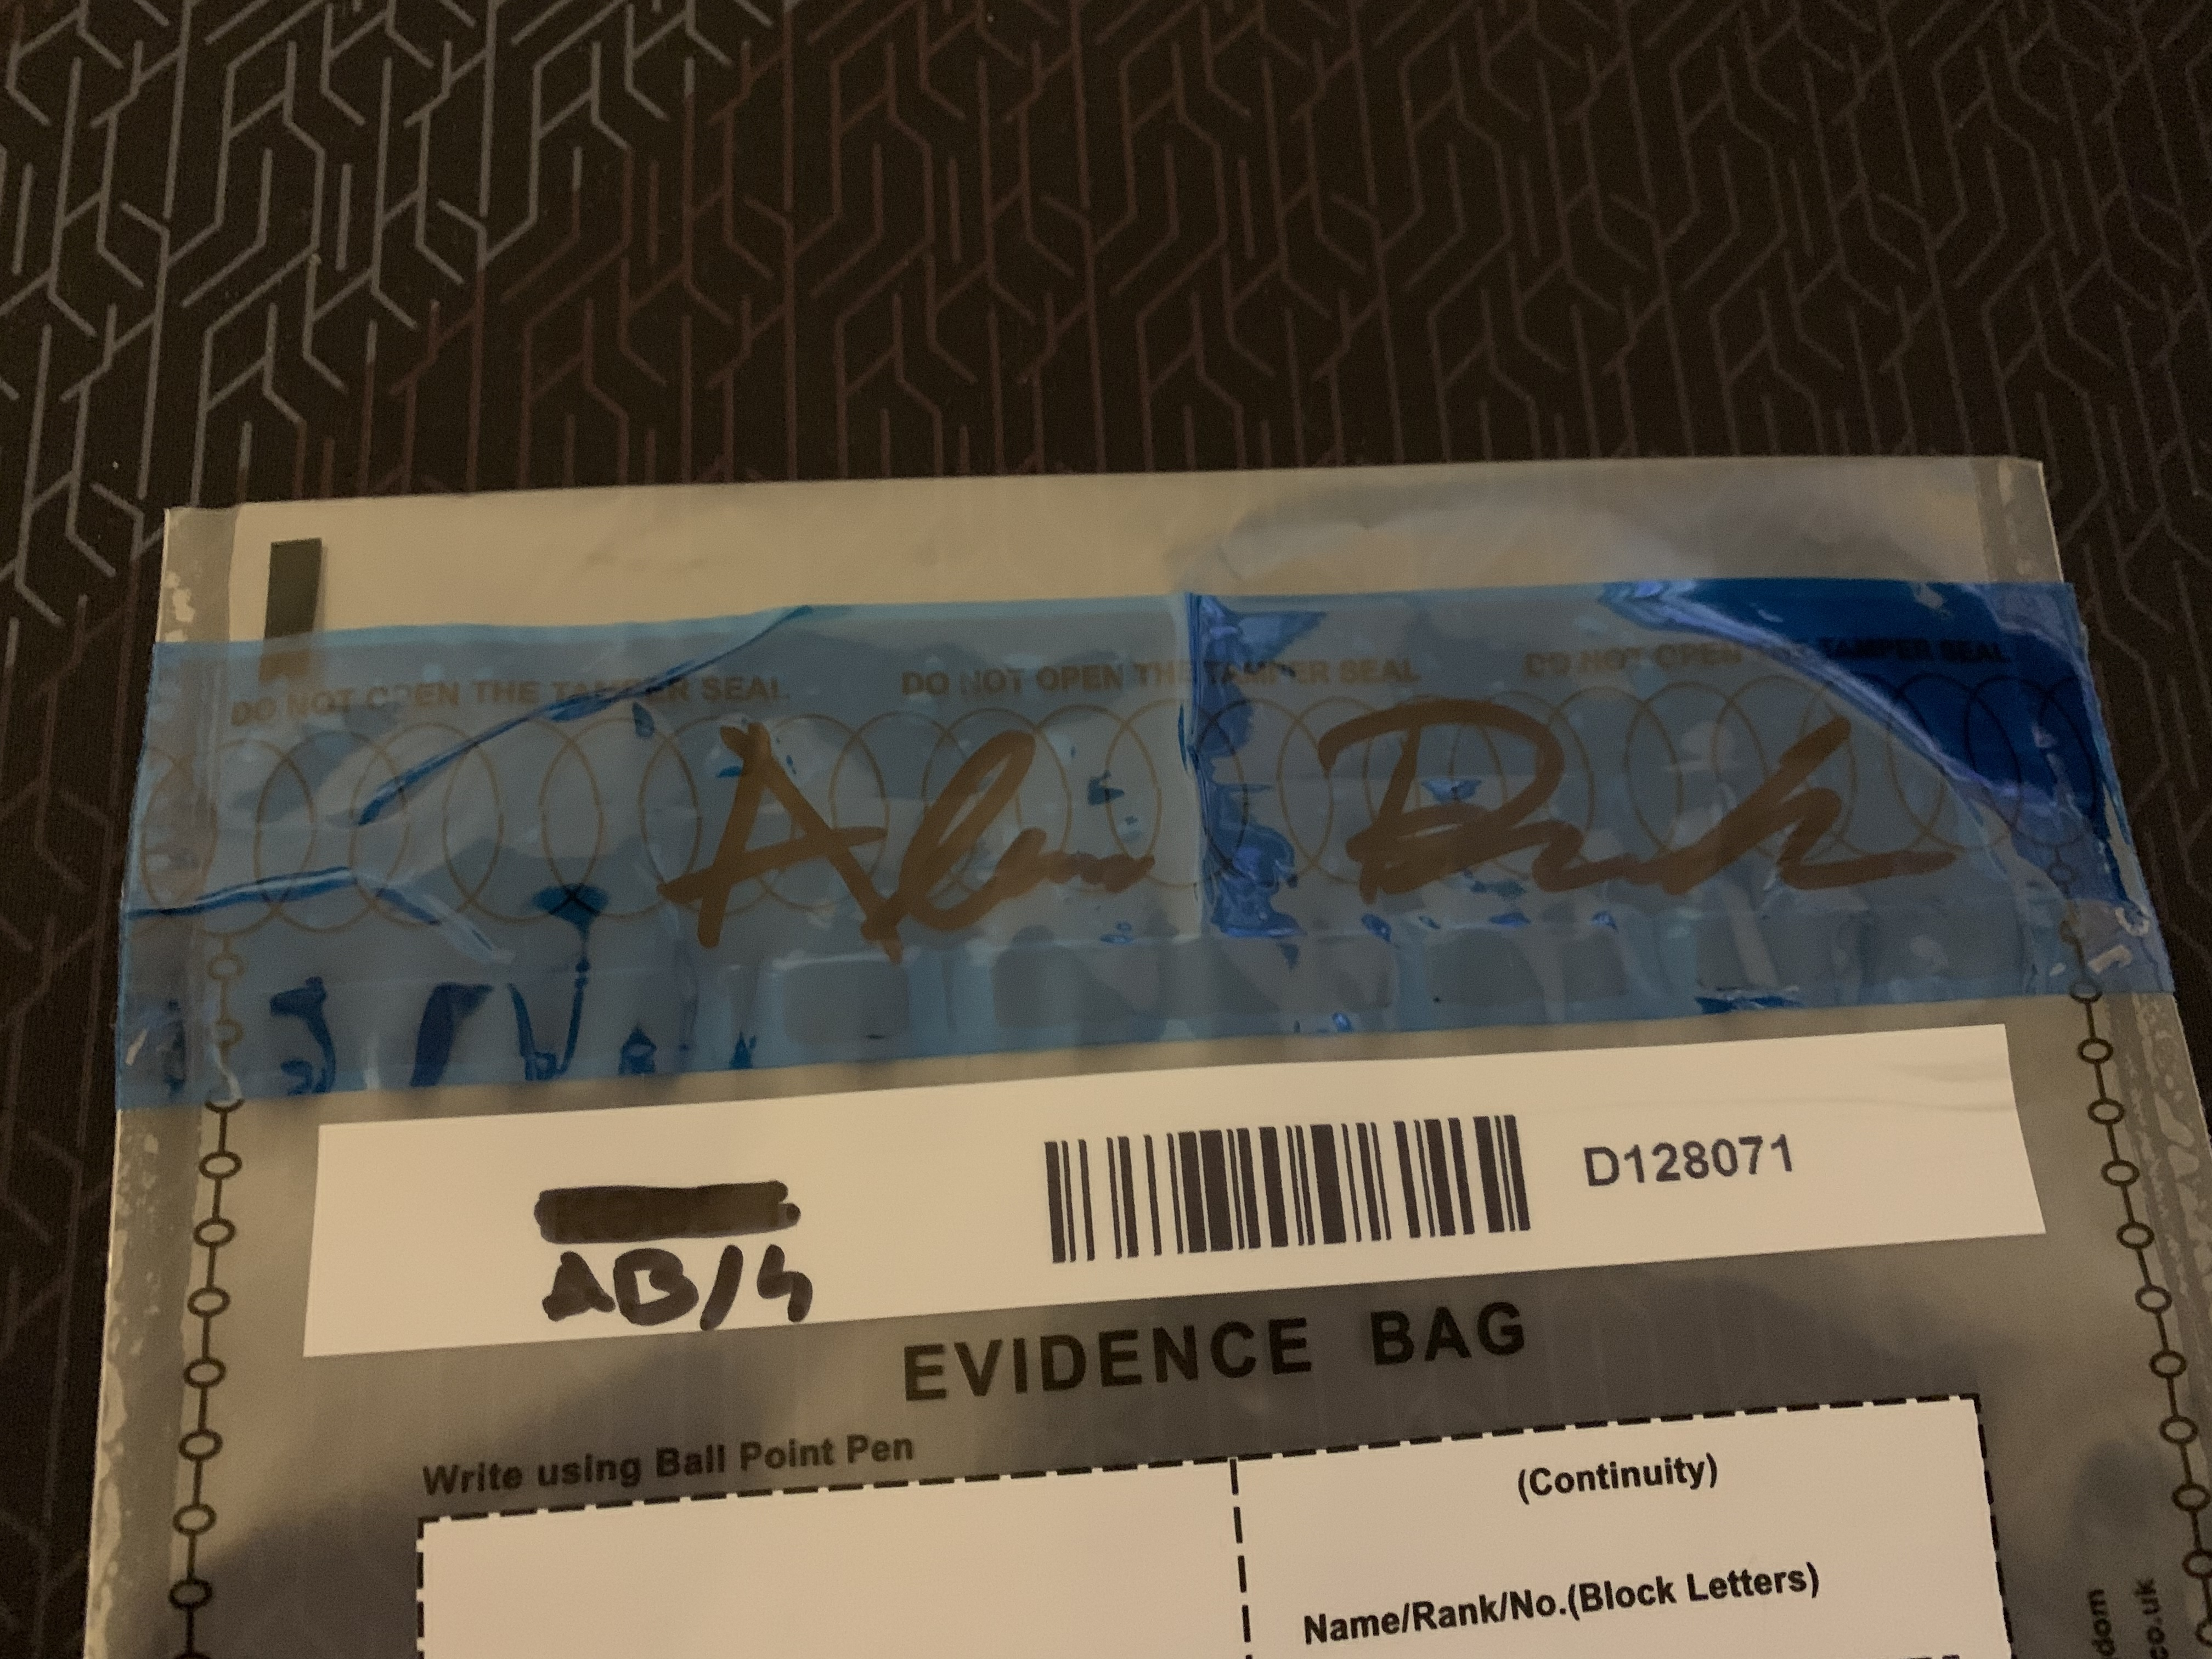
\includegraphics[width=0.7\textwidth]{figures/pictures/IMG_5055.JPG}
  \caption{Close-up Seal}
  \label{fig:closeup}
\end{figure}

This is an example of possible tempered evidence.
\label{s:broken-seal}
\begin{figure}[h]
  \centering
  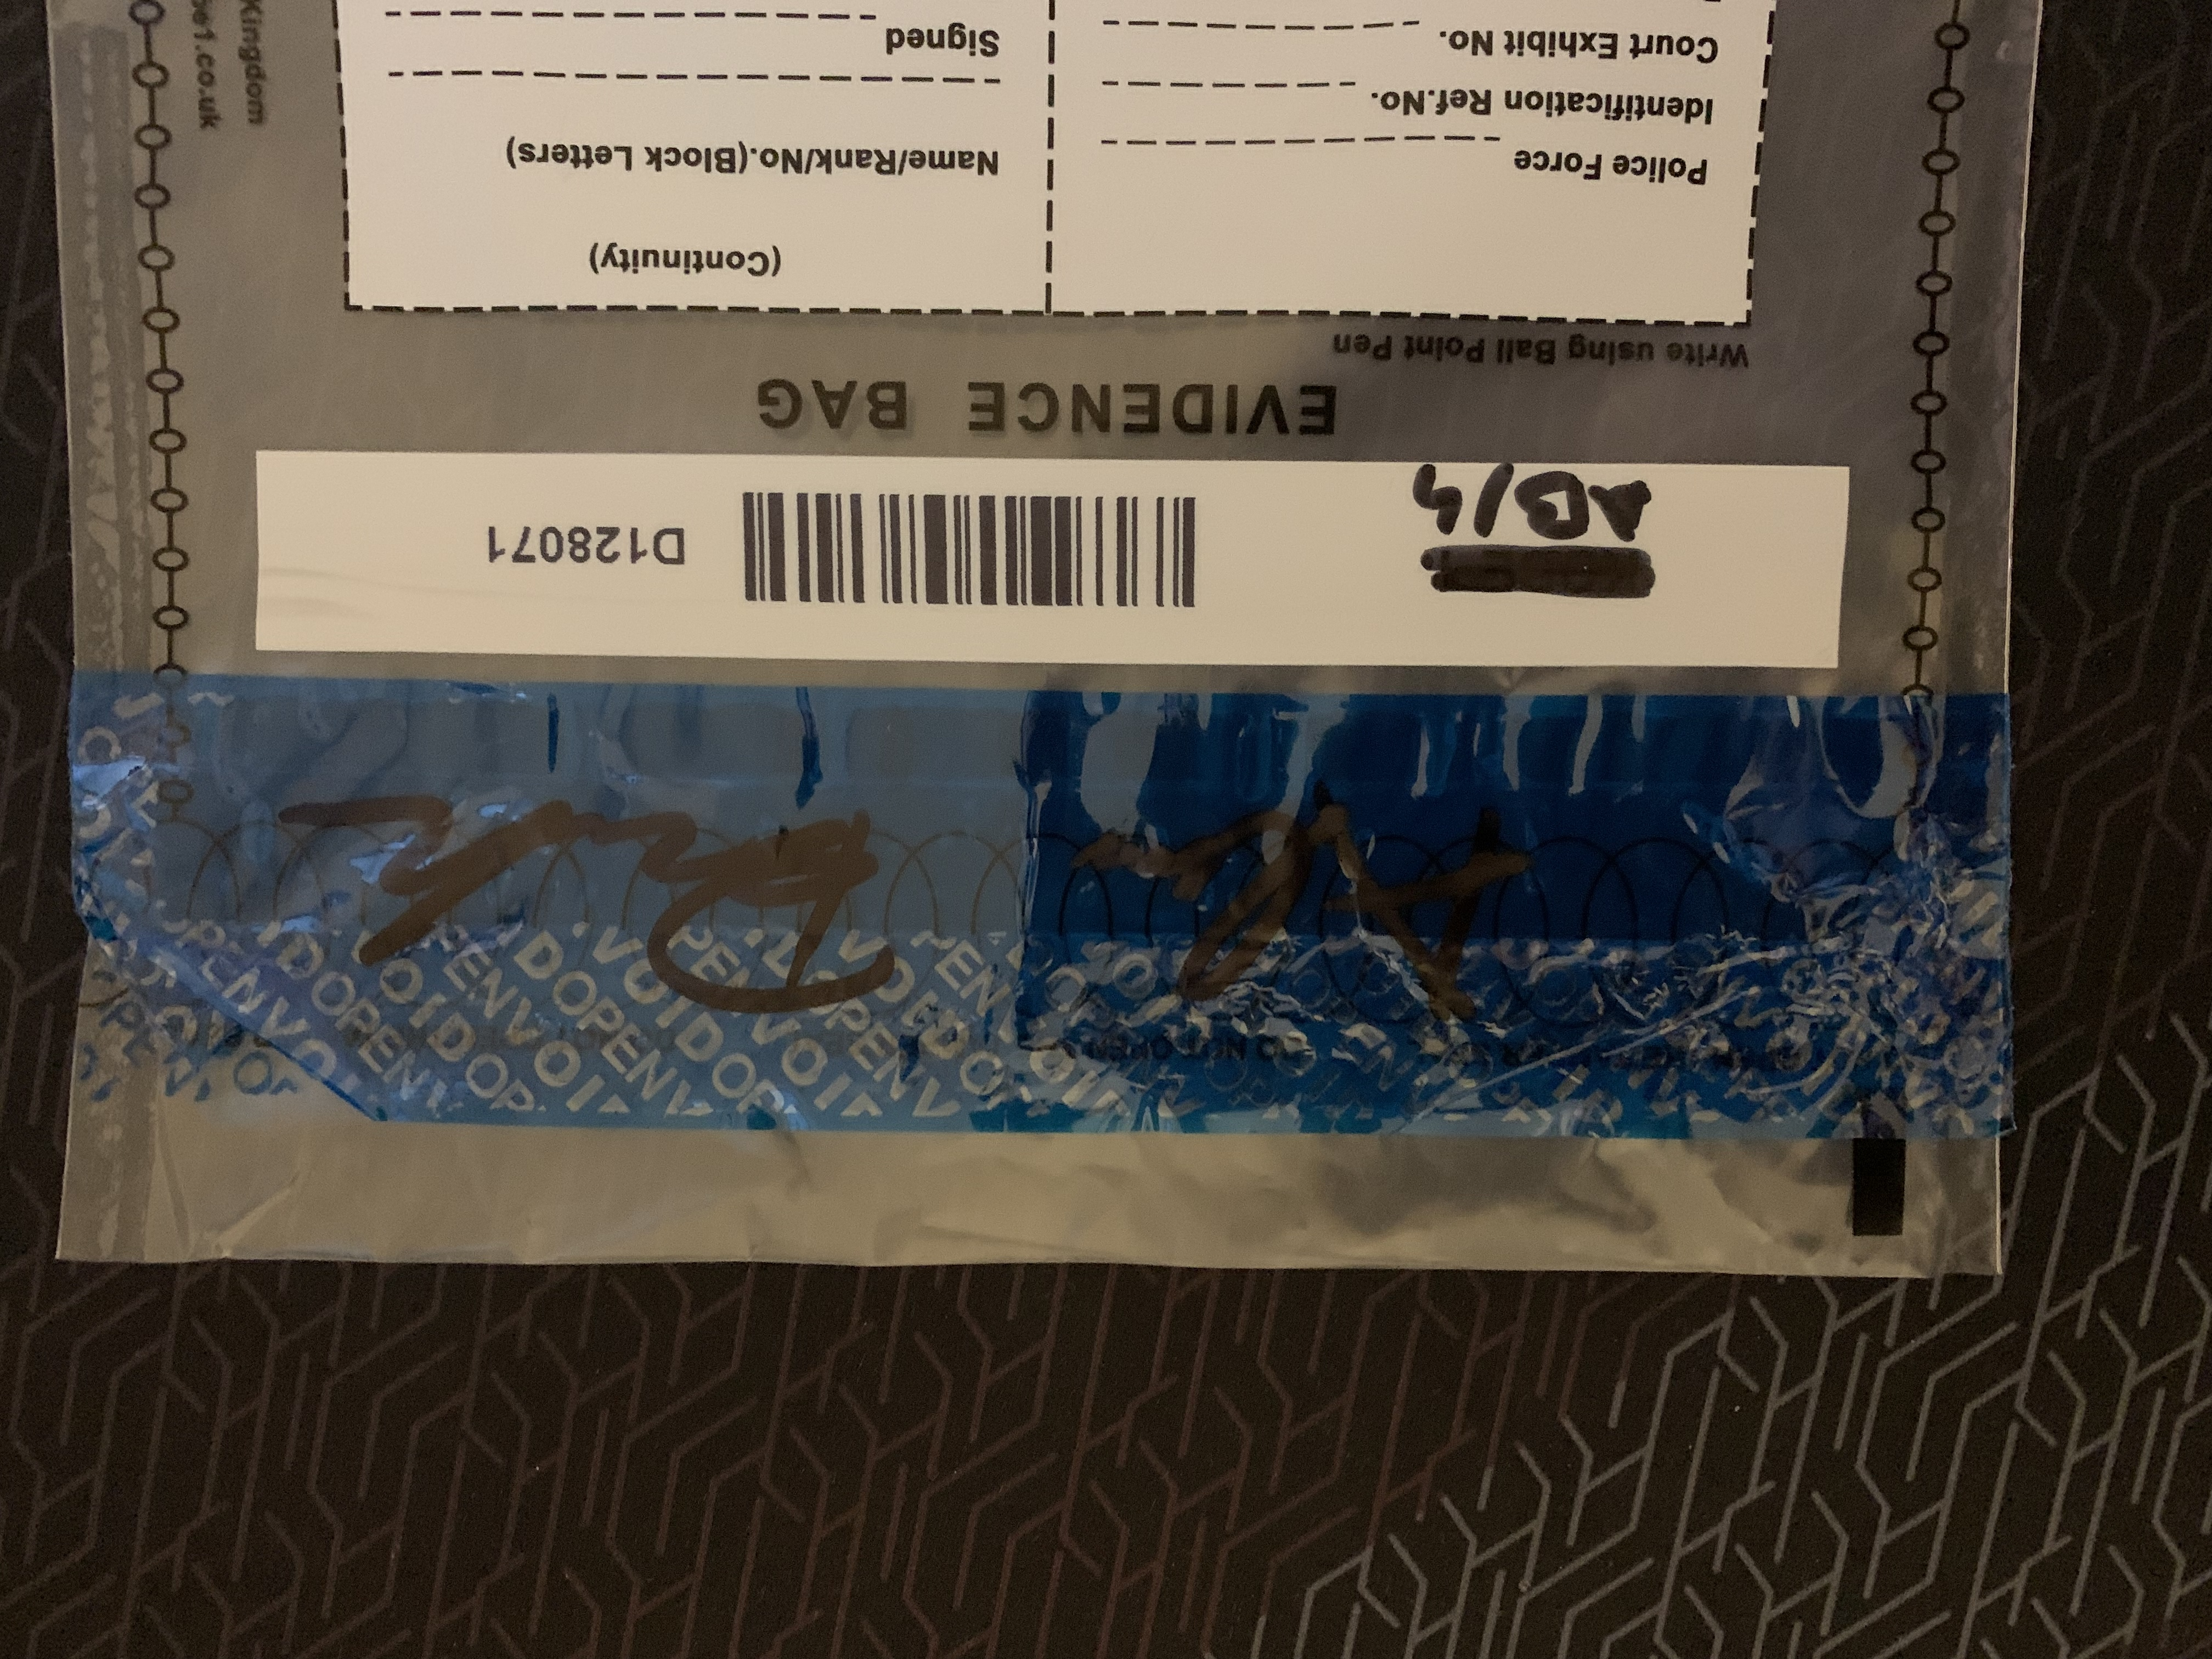
\includegraphics[width=0.7\textwidth, angle=180,origin=c]{figures/pictures/IMG_5059.JPG}
  \caption{Broken Seal}
  \label{fig:broken}
\end{figure}
\newpage
